\hypertarget{animal-locomotion-and-support-systems}{%
\chapter{Animal Locomotion And Support Systems}\label{animal-locomotion-and-support-systems}}

Animal locomotion is any of a variety of methods that animals use to move from one place to another. Some modes of locomotion are (initially) self-propelled, e.g., running, swimming, jumping, flying, hopping, soaring and gliding. There are also many animal species that depend on their environment for transportation, a type of mobility called passive locomotion, e.g., sailing (some jellyfish), kiting (spiders), rolling (some beetles and spiders) or riding other animals (phoresis).

The term ``locomotion'' is formed in English from Latin loco ``from a place'' (ablative of locus ``place'') + motio ``motion, a moving''.

Animals move for a variety of reasons, such as to find food, a mate, a suitable microhabitat, or to escape predators. For many animals, the ability to move is essential for survival and, as a result, natural selection has shaped the locomotion methods and mechanisms used by moving organisms. For example, migratory animals that travel vast distances (such as the Arctic tern) typically have a locomotion mechanism that costs very little energy per unit distance, whereas non-migratory animals that must frequently move quickly to escape predators are likely to have energetically costly, but very fast, locomotion.

The anatomical structures that animals use for movement, including cilia, legs, wings, arms, fins, or tails are sometimes referred to as locomotory organs or locomotory structures.

Animals move through, or on, four types of environment: aquatic (in or on water), terrestrial (on ground or other surface, including arboreal, or tree-dwelling), fossorial (underground), and aerial (in the air). Many animals---for example semi-aquatic animals, and diving birds---regularly move through more than one type of medium. In some cases, the surface they move on facilitates their method of locomotion.

\hypertarget{the-skeleton}{%
\section{The Skeleton}\label{the-skeleton}}

The skeleton is the body part that provides support, shape and protection to the soft tissues and delicate organs of animals. There are several different skeletal types: the exoskeleton, which is the stable outer shell of an organism, the endoskeleton, which forms the support structure inside the body, the hydroskeleton, a flexible skeleton supported by fluid pressure, and the cytoskeleton present in the cytoplasm of all cells, including bacteria, and archaea. The term comes from Greek σκελετός (skeletós), meaning `dried up'.

There are two major types of skeletons: solid and fluid. Solid skeletons can be internal, called an endoskeleton, or external, called an exoskeleton, and may be further classified as pliant (elastic/movable) or rigid (hard/non-movable). Fluid skeletons are always internal.

\hypertarget{exoskeleton}{%
\subsection{Exoskeleton}\label{exoskeleton}}

Exoskeletons are external, and are found in many invertebrates; they enclose and protect the soft tissues and organs of the body. Some kinds of exoskeletons undergo periodic moulting or ecdysis as the animal grows, as is the case in many arthropods including insects and crustaceans.

The exoskeleton of insects is not only a form of protection, but also serves as a surface for muscle attachment, as a watertight protection against drying, and as a sense organ to interact with the environment. The shell of mollusks also performs all of the same functions, except that in most cases it does not contain sense organs.

An external skeleton can be quite heavy in relation to the overall mass of an animal, so on land, organisms that have an exoskeleton are mostly relatively small. Somewhat larger aquatic animals can support an exoskeleton because weight is less of a consideration underwater. The southern giant clam, a species of extremely large saltwater clam in the Pacific Ocean, has a shell that is massive in both size and weight. Syrinx aruanus is a species of sea snail with a very large shell.

\hypertarget{endoskeleton}{%
\subsection{Endoskeleton}\label{endoskeleton}}

The endoskeleton is the internal support structure of an animal, composed of mineralized tissue and is typical of vertebrates. Endoskeletons vary in complexity from functioning purely for support (as in the case of sponges), to serving as an attachment site for muscles and a mechanism for transmitting muscular forces. A true endoskeleton is derived from mesodermal tissue. Such a skeleton is present in echinoderms and chordates.



\begin{figure}

{\centering 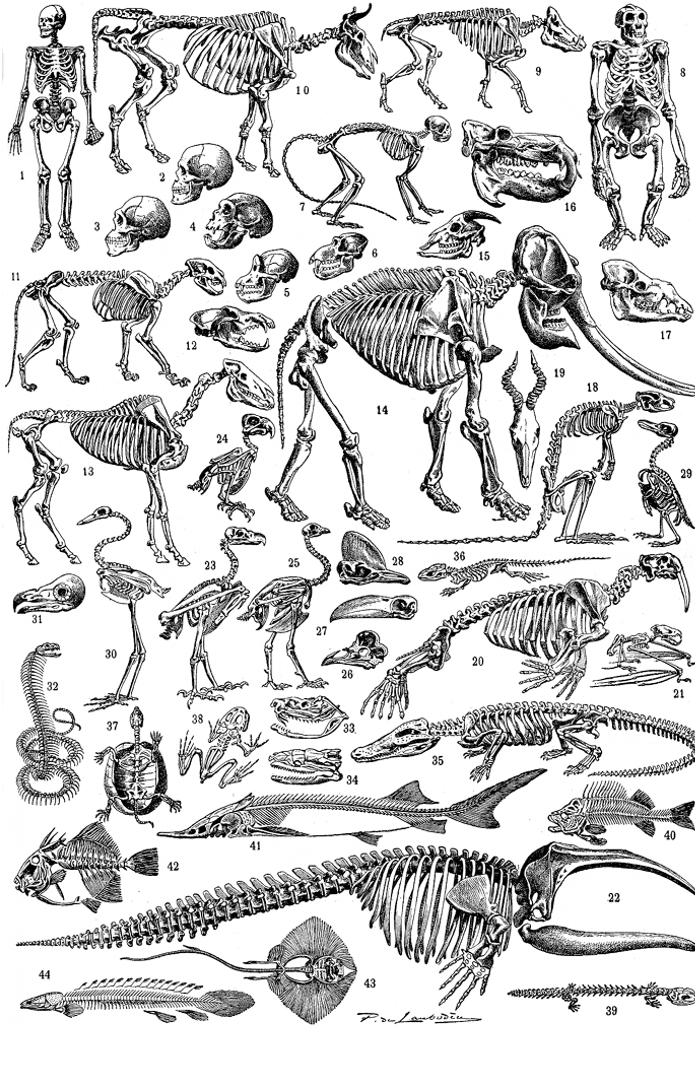
\includegraphics[width=0.7\linewidth]{./figures/locomotion/Skeletons} 

}

\caption{\href{https://upload.wikimedia.org/wikipedia/commons/8/87/Skeletons.png}{Vertebrate skulls and skeletons}: 1. \href{https://commons.wikimedia.org/wiki/File:S,keleton_diagram.svg}{Homo sapiens}, 2. \href{https://commons.wikimedia.org/wiki/File:Gray188_skull_left_lateral_index.png}{Human skull}, 3. \href{https://commons.wikimedia.org/wiki/File:Australopithecus.jpg}{Australopithecus}, 4. \href{https://commons.wikimedia.org/wiki/File:Homo_sapiens_neanderthalensis.jpg}{Homo neanderthalensis}, 5. \href{https://commons.wikimedia.org/wiki/File:Pan_troglodytes01.jpg}{Pan troglodytes}, 6. \href{https://commons.wikimedia.org/wiki/File:Huxley_-_Mans_Place_in_Nature.jpg}{Papio hamadryas}, 7. \href{https://commons.wikimedia.org/wiki/File:Goldstumpfnasen_(Rhinopithecus_roxellana).jpg}{Rhinopithecus roxellan}, 8. \href{https://commons.wikimedia.org/wiki/File:GorillaSkeleton.jpg}{Gorilla}, 9. \href{https://commons.wikimedia.org/wiki/File:PigSkelLyd2.png}{Sus scrofa}, 10. \href{https://commons.wikimedia.org/wiki/File:Heubach_cattle_skull.jpg}{Cattle}, 11. \href{https://commons.wikimedia.org/wiki/File:Lion_anatomy_lateral_skeleton_view.jpg}{Panthera leo}, 12. \href{https://commons.wikimedia.org/wiki/File:WolfSkelLyd1.png}{Canis lupus}, 13. \href{https://commons.wikimedia.org/wiki/File:Horse_bones_ugglan.jpg}{Equus caballus}, 14. \href{https://commons.wikimedia.org/wiki/File:ElephantSkelLyd2.png}{Elephantidae}, 15. \href{https://commons.wikimedia.org/wiki/File:Goat_anatomy_lateral_skeleton_view.jpg}{Capra}, 16. \href{https://commons.wikimedia.org/wiki/File:HippoSkelLyd2.png}{Hippopotamus}, 17. \href{https://commons.wikimedia.org/wiki/File:CamelSkelLyd2.png}{Camelus}, 18. \href{https://commons.wikimedia.org/wiki/File:Macropodidae_skeleton.png}{Macropus}, 19. \href{https://commons.wikimedia.org/wiki/File:ChausinghaSkullLyd2.png}{Damaliscus korrigum}, 20. \href{https://commons.wikimedia.org/wiki/File:WalrusLyd2.png}{Odobenus rosmarus}, 21. \href{https://commons.wikimedia.org/wiki/File:Fledermaus_(Nycteris_fuliginosis).png}{Bat}, 22. \href{https://commons.wikimedia.org/wiki/File:GreenlandWhaleLyd3.jpg}{Cetacea}, 23. \href{https://commons.wikimedia.org/wiki/File:Baldeagle-06jul16.jpg}{Accipitridae}, 24. \href{https://commons.wikimedia.org/wiki/File:ParrotSkelLyd.jpg}{Psittacidae}, 25. \href{https://commons.wikimedia.org/wiki/File:Furcula.png}{Gallus gallus}, 26. \href{https://commons.wikimedia.org/wiki/File:Furcula.png}{Roosters}, 27. \href{https://commons.wikimedia.org/wiki/File:Toco_toucan_whipsnade.jpg}{Ramphastos sulfuratus}, 28. \href{https://commons.wikimedia.org/wiki/File:CassowarySkullLyd4.png}{Casuariidae}, 29. \href{https://commons.wikimedia.org/wiki/File:Skull_alca_torda.jpg}{Spheniscidae}, 30. \href{https://commons.wikimedia.org/wiki/File:Grus_grus_skull.png}{Gruidae}, 32. \href{https://commons.wikimedia.org/wiki/File:Sharovipteryx_BW.jpg}{Sharovipteryx mirabilis}, 32. \href{https://commons.wikimedia.org/wiki/File:Python_gab_fbi.png}{Natrix natrix}, 33. \href{}{Crotalinae}, 34. \href{https://commons.wikimedia.org/wiki/File:Acrantophis_dumerili.jpg}{Boa constrictor}, 35. \href{https://commons.wikimedia.org/wiki/File:Crocodilelyd5.png}{Crocodile}, 36. \href{https://commons.wikimedia.org/wiki/File:Pleurodont_jaw_Mivart.png}{Lizard}, 37. \href{https://commons.wikimedia.org/wiki/File:SmithTestudoSkeletonTagged.PNG}{Testudines}, 38. \href{https://commons.wikimedia.org/wiki/File:Rana_skull.png}{Frog}, 39. \href{https://commons.wikimedia.org/wiki/File:Albanerpeton_BW.jpg}{Salamandra salamandra}, 40. \href{https://commons.wikimedia.org/wiki/File:Pesce_Persico.jpg}{Perca fluviatilis}, 41. \href{https://commons.wikimedia.org/wiki/File:Sturgeon2.jpg}{Acipenser}, 42. \href{https://commons.wikimedia.org/wiki/Category:Balistoides_viridescens}{Balistoides viridescens}, 43. \href{https://commons.wikimedia.org/wiki/File:Smooth_skate.jpg}{Rajidae}, 44. \href{https://commons.wikimedia.org/wiki/Category:Polypterus}{Polypterus}}\label{fig:skullskeletons}
\end{figure}

Pliant skeletons are capable of movement; thus, when stress is applied to the skeletal structure, it deforms and then reverts to its original shape. This skeletal structure is used in some invertebrates, for instance in the hinge of bivalve shells or the mesoglea of cnidarians such as jellyfish. Pliant skeletons are beneficial because only muscle contractions are needed to bend the skeleton; upon muscle relaxation, the skeleton will return to its original shape. Cartilage is one material that a pliant skeleton may be composed of, but most pliant skeletons are formed from a mixture of proteins, polysaccharides, and water. For additional structure or protection, pliant skeletons may be supported by rigid skeletons. Organisms that have pliant skeletons typically live in water, which supports body structure in the absence of a rigid skeleton.

Rigid skeletons are not capable of movement when stressed, creating a strong support system most common in terrestrial animals. Such a skeleton type used by animals that live in water are more for protection (such as barnacle and snail shells) or for fast-moving animals that require additional support of musculature needed for swimming through water. Rigid skeletons are formed from materials including chitin (in arthropods), calcium compounds such as calcium carbonate (in stony corals and mollusks) and silicate (for diatoms and radiolarians).

\hypertarget{hydrostatic-skeleton-hydroskeleton}{%
\subsection{Hydrostatic Skeleton (Hydroskeleton)}\label{hydrostatic-skeleton-hydroskeleton}}

A hydrostatic skeleton is a semi-rigid, soft tissue structure filled with liquid under pressure, surrounded by muscles. Longitudinal and circular muscles around their body sectors allow movement by alternate lengthening and contractions along their lengths. A common example of this is the earthworm.

\hypertarget{organisms-with-skeletons}{%
\subsection{Organisms With Skeletons}\label{organisms-with-skeletons}}

The endoskeletons of echinoderms and some other soft-bodied invertebrates such as jellyfish and earthworms are also termed hydrostatic; a body cavity the coelom is filled with coelomic fluid and the pressure from this fluid acts together with the surrounding muscles to change the organism's shape and produce movement.

The skeleton of sponges consists of microscopic calcareous or silicious spicules. The demosponges include 90\% of all species of sponges. Their ``skeletons'' are made of spicules consisting of fibers of the protein spongin, the mineral silica, or both. Where spicules of silica are present, they have a different shape from those in the otherwise similar glass sponges.

The skeleton of the echinoderms, which include, among other things, the starfish, is composed of calcite and a small amount of magnesium oxide. It lies below the epidermis in the mesoderm and is within cell clusters of frame-forming cells. This structure formed is porous and therefore firm and at the same time light. It coalesces into small calcareous ossicles (bony plates), which can grow in all directions and thus can replace the loss of a body part. Connected by joints, the individual skeletal parts can be moved by the muscles.

In most vertebrates, the main skeletal component is referred to as bone. These bones compose a unique skeletal system for each type of animal. Another important component is cartilage which in mammals is found mainly in the joint areas. In other animals, such as the cartilaginous fishes, which include the sharks, the skeleton is composed entirely of cartilage. The segmental pattern of the skeleton is present in all vertebrates (mammals, birds, fish, reptiles and amphibians) with basic units being repeated. This segmental pattern is particularly evident in the vertebral column and the ribcage.

Bones in addition to supporting the body also serve, at the cellular level, as calcium and phosphate storage.

The skeleton, which forms the support structure inside the fish is either made of cartilage as in the (Chondrichthyes), or bones as in the (Osteichthyes). The main skeletal element is the vertebral column, composed of articulating vertebrae which are lightweight yet strong. The ribs attach to the spine and there are no limbs or limb girdles. They are supported only by the muscles. The main external features of the fish, the fins, are composed of either bony or soft spines called rays, which with the exception of the caudal fin (tail fin), have no direct connection with the spine. They are supported by the muscles which compose the main part of the trunk.

The bird skeleton is highly adapted for flight. It is extremely lightweight, yet still strong enough to withstand the stresses of taking off, flying, and landing. One key adaptation is the fusing of bones into single ossifications, such as the pygostyle. Because of this, birds usually have a smaller number of bones than other terrestrial vertebrates. Birds also lack teeth or even a true jaw, instead having evolved a beak, which is far more lightweight. The beaks of many baby birds have a projection called an egg tooth, which facilitates their exit from the amniotic egg.

\hypertarget{the-human-musculoskeletal-system}{%
\section{The Human Musculoskeletal System}\label{the-human-musculoskeletal-system}}

The human musculoskeletal system (also known as the locomotor system, and previously the activity system) is an organ system that gives humans the ability to move using their muscular and skeletal systems. The musculoskeletal system provides form, support, stability, and movement to the body.

It is made up of the bones of the skeleton, muscles, cartilage, tendons, ligaments, joints, and other connective tissue that supports and binds tissues and organs together. The musculoskeletal system's primary functions include supporting the body, allowing motion, and protecting vital organs. The skeletal portion of the system serves as the main storage system for calcium and phosphorus and contains critical components of the hematopoietic system.

This system describes how bones are connected to other bones and muscle fibers via connective tissue such as tendons and ligaments. The bones provide stability to the body. Muscles keep bones in place and also play a role in the movement of bones. To allow motion, different bones are connected by joints. Cartilage prevents the bone ends from rubbing directly onto each other. Muscles contract to move the bone attached at the joint.

There are, however, diseases and disorders that may adversely affect the function and overall effectiveness of the system. These diseases can be difficult to diagnose due to the close relation of the musculoskeletal system to other internal systems. The musculoskeletal system refers to the system having its muscles attached to an internal skeletal system and is necessary for humans to move to a more favorable position. Complex issues and injuries involving the musculoskeletal system are usually handled by a physiatrist (specialist in physical medicine and rehabilitation) or an orthopaedic surgeon.

The skeletal system serves many important functions; it provides the shape and form for the body, support and protection, allows bodily movement, produces blood for the body, and stores minerals. The number of bones in the human skeletal system is a controversial topic. Humans are born with over 300 bones; however, many bones fuse together between birth and maturity. As a result, an average adult skeleton consists of 206 bones. The number of bones varies according to the method used to derive the count. While some consider certain structures to be a single bone with multiple parts, others may see it as a single part with multiple bones. There are five general classifications of bones. These are long bones, short bones, flat bones, irregular bones, and sesamoid bones. The human skeleton is composed of both fused and individual bones supported by ligaments, tendons, muscles and cartilage. It is a complex structure with two distinct divisions; the axial skeleton, which includes the vertebral column, and the appendicular skeleton.

The skeletal system serves as a framework for tissues and organs to attach themselves to. This system acts as a protective structure for vital organs. Major examples of this are the brain being protected by the skull and the lungs being protected by the rib cage.

Located in long bones are two distinctions of bone marrow (yellow and red). The yellow marrow has fatty connective tissue and is found in the marrow cavity. During starvation, the body uses the fat in yellow marrow for energy. The red marrow of some bones is an important site for blood cell production, approximately 2.6 million red blood cells per second in order to replace existing cells that have been destroyed by the liver. Here all erythrocytes, platelets, and most leukocytes form in adults. From the red marrow, erythrocytes, platelets, and leukocytes migrate to the blood to do their special tasks.

Another function of bones is the storage of certain minerals. Calcium and phosphorus are among the main minerals being stored. The importance of this storage ``device'' helps to regulate mineral balance in the bloodstream. When the fluctuation of minerals is high, these minerals are stored in bone; when it is low it will be withdrawn from the bone.

There are three types of muscles---cardiac, skeletal, and smooth. Smooth muscles are used to control the flow of substances within the lumens of hollow organs, and are not consciously controlled. Skeletal and cardiac muscles have striations that are visible under a microscope due to the components within their cells. Only skeletal and smooth muscles are part of the musculoskeletal system and only the skeletal muscles can move the body. Cardiac muscles are found in the heart and are used only to circulate blood; like the smooth muscles, these muscles are not under conscious control. Skeletal muscles are attached to bones and arranged in opposing groups around joints. Muscles are innervated, to communicate nervous energy to, by nerves, which conduct electrical currents from the central nervous system and cause the muscles to contract.

In mammals, when a muscle contracts, a series of reactions occur. Muscle contraction is stimulated by the motor neuron sending a message to the muscles from the somatic nervous system. Depolarization of the motor neuron results in neurotransmitters being released from the nerve terminal. The space between the nerve terminal and the muscle cell is called the neuromuscular junction. These neurotransmitters diffuse across the synapse and bind to specific receptor sites on the cell membrane of the muscle fiber. When enough receptors are stimulated, an action potential is generated and the permeability of the sarcolemma is altered. This process is known as initiation.

\hypertarget{tendons}{%
\subsection{Tendons}\label{tendons}}

A tendon is a tough, flexible band of fibrous connective tissue that connects muscles to bones. The extra-cellular connective tissue between muscle fibers binds to tendons at the distal and proximal ends, and the tendon binds to the periosteum of individual bones at the muscle's origin and insertion. As muscles contract, tendons transmit the forces to the relatively rigid bones, pulling on them and causing movement. Tendons can stretch substantially, allowing them to function as springs during locomotion, thereby saving energy.

\hypertarget{joints-ligaments-and-bursae}{%
\subsection{Joints, Ligaments And Bursae}\label{joints-ligaments-and-bursae}}

Joints are structures that connect individual bones and may allow bones to move against each other to cause movement. There are three divisions of joints, diarthroses which allow extensive mobility between two or more articular heads; amphiarthrosis, which is a joint that allows some movement, and false joints or synarthroses, joints that are immovable, that allow little or no movement and are predominantly fibrous. Synovial joints, joints that are not directly joined, are lubricated by a solution called synovial fluid that is produced by the synovial membranes. This fluid lowers the friction between the articular surfaces and is kept within an articular capsule, binding the joint with its taut tissue.



\begin{figure}

{\centering 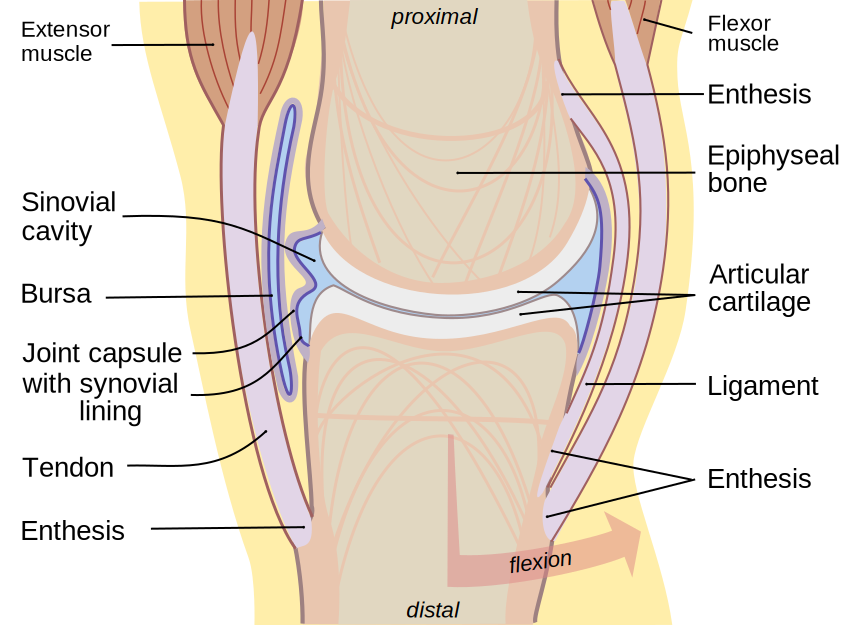
\includegraphics[width=0.7\linewidth]{./figures/locomotion/Joint} 

}

\caption{\href{https://commons.wikimedia.org/wiki/File:Joint.svg}{A synovial joint.}}\label{fig:synovialjoint}
\end{figure}

A ligament is a small band of dense, white, fibrous elastic tissue. Ligaments connect the ends of bones together in order to form a joint. Most ligaments limit dislocation, or prevent certain movements that may cause breaks. Since they are only elastic they increasingly lengthen when under pressure. When this occurs the ligament may be susceptible to break resulting in an unstable joint.



\begin{figure}

{\centering 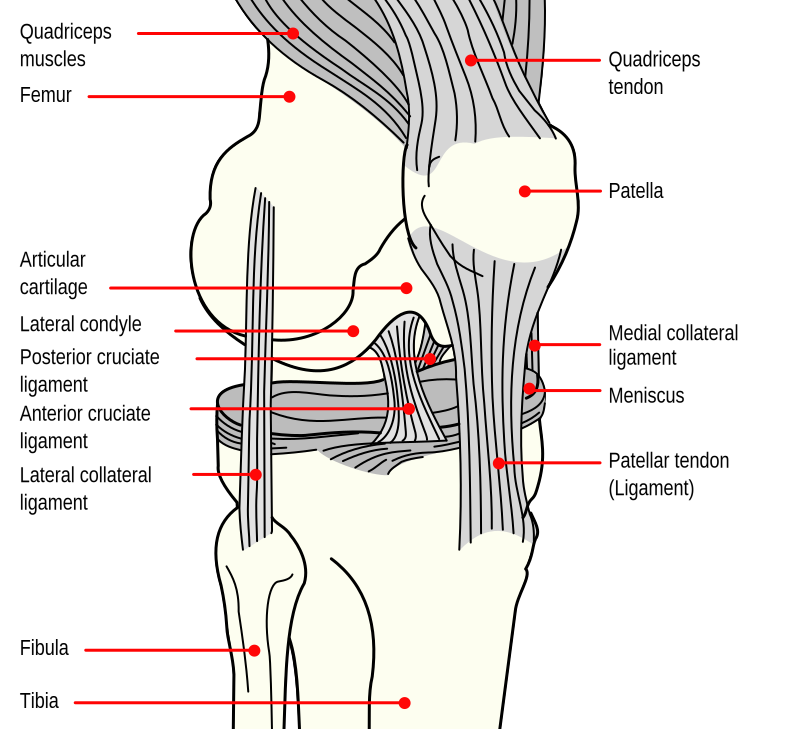
\includegraphics[width=0.7\linewidth]{./figures/locomotion/Knee_diagram} 

}

\caption{\href{https://commons.wikimedia.org/wiki/File:Knee_diagram.svg}{Diagram of the right knee. Anterior cruciate ligament labeled at center left.}}\label{fig:kneeligaments}
\end{figure}

Ligaments may also restrict some actions: movements such as hyper extension and hyper flexion are restricted by ligaments to an extent. Also ligaments prevent certain directional movement.

A bursa is a small fluid-filled sac made of white fibrous tissue and lined with synovial membrane. Bursa may also be formed by a synovial membrane that extends outside of the joint capsule. It provides a cushion between bones and tendons or muscles around a joint; bursa are filled with synovial fluid and are found around almost every major joint of the body.

\hypertarget{the-human-skeleton}{%
\subsection{The Human Skeleton}\label{the-human-skeleton}}

The human skeleton consists of both fused and individual bones supported and supplemented by ligaments, tendons, muscles and cartilage. It is composed of around 270 bones at birth -- this total decreases to around 206 bones by adulthood after some bones get fused together. The biggest bone in the body is the femur in the upper leg, and the smallest is the stapes bone in the middle ear. In an adult, the skeleton comprises around 14\% of the total body weight, and half of this weight is water. The bone mass in the skeleton reaches maximum density around age 21. The human skeleton can be divided into the axial skeleton and the appendicular skeleton. The axial skeleton is formed by the vertebral column, the rib cage, the skull and other associated bones. The appendicular skeleton, which is attached to the axial skeleton, is formed by the shoulder girdle, the pelvic girdle and the bones of the upper and lower limbs.



\begin{figure}

{\centering 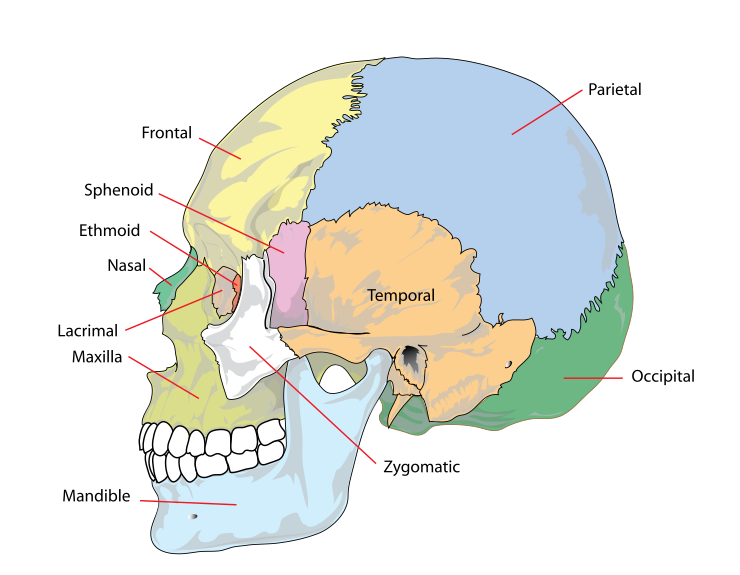
\includegraphics[width=0.7\linewidth]{./figures/locomotion/Human_skull_side_simplified_(bones)} 

}

\caption{\href{https://commons.wikimedia.org/wiki/File:Human_skull_side_simplified_(bones).svg}{Major bones of the human skull viewed from the side.}}\label{fig:humanskull}
\end{figure}

The human skeleton performs six major functions; support, movement, protection, production of blood cells, storage of minerals, and endocrine regulation.It serves as a scaffold which supports organs, anchors muscles, and protects organs such as the brain, lungs, heart and spinal cord. Although the teeth do not consist of tissue commonly found in bones, the teeth are usually considered as members of the skeletal system.

Fused bones include those of the pelvis and the cranium. Not all bones are interconnected directly: There are three bones in each middle ear called the ossicles that articulate only with each other. The hyoid bone, which is located in the neck and serves as the point of attachment for the tongue, does not articulate with any other bones in the body, being supported by muscles and ligaments.



\begin{figure}

{\centering 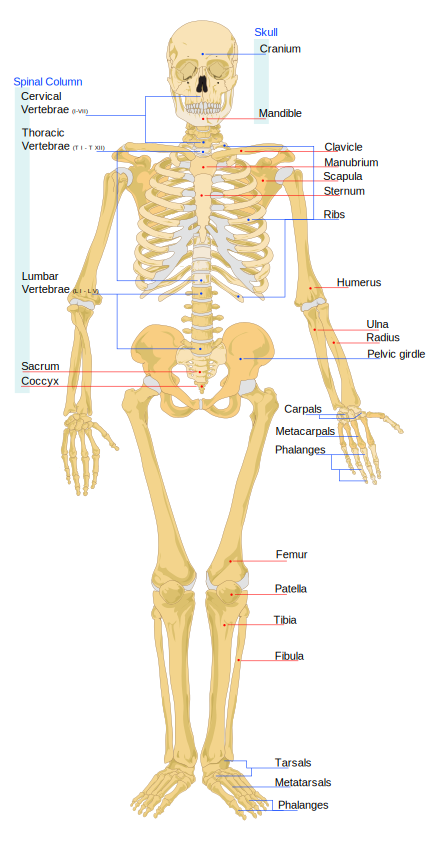
\includegraphics[width=0.7\linewidth]{./figures/locomotion/Human_skeleton_front_en} 

}

\caption{\href{https://commons.wikimedia.org/wiki/File:Human_skeleton_front_en.svg}{The human skeleton viewed from the front.}}\label{fig:humanskeletonfront}
\end{figure}

There are 206 bones in the adult human skeleton, although this number depends on whether the pelvic bones (the hip bones on each side) are counted as one or three bones on each side (ilium, ischium, and pubis), whether the coccyx or tail bone is counted as one or four separate bones, and does not count the variable wormian bones between skull sutures. Similarly, the sacrum is usually counted as a single bone, rather than five fused vertebrae. There is also a variable number of small sesamoid bones, commonly found in tendons. The patella or kneecap on each side is an example of a larger sesamoid bone. The patellae are counted in the total, as they are constant. The number of bones varies between individuals and with age -- newborn babies have over 270 bones some of which fuse together. These bones are organized into a longitudinal axis, the axial skeleton, to which the appendicular skeleton is attached.



\begin{figure}

{\centering 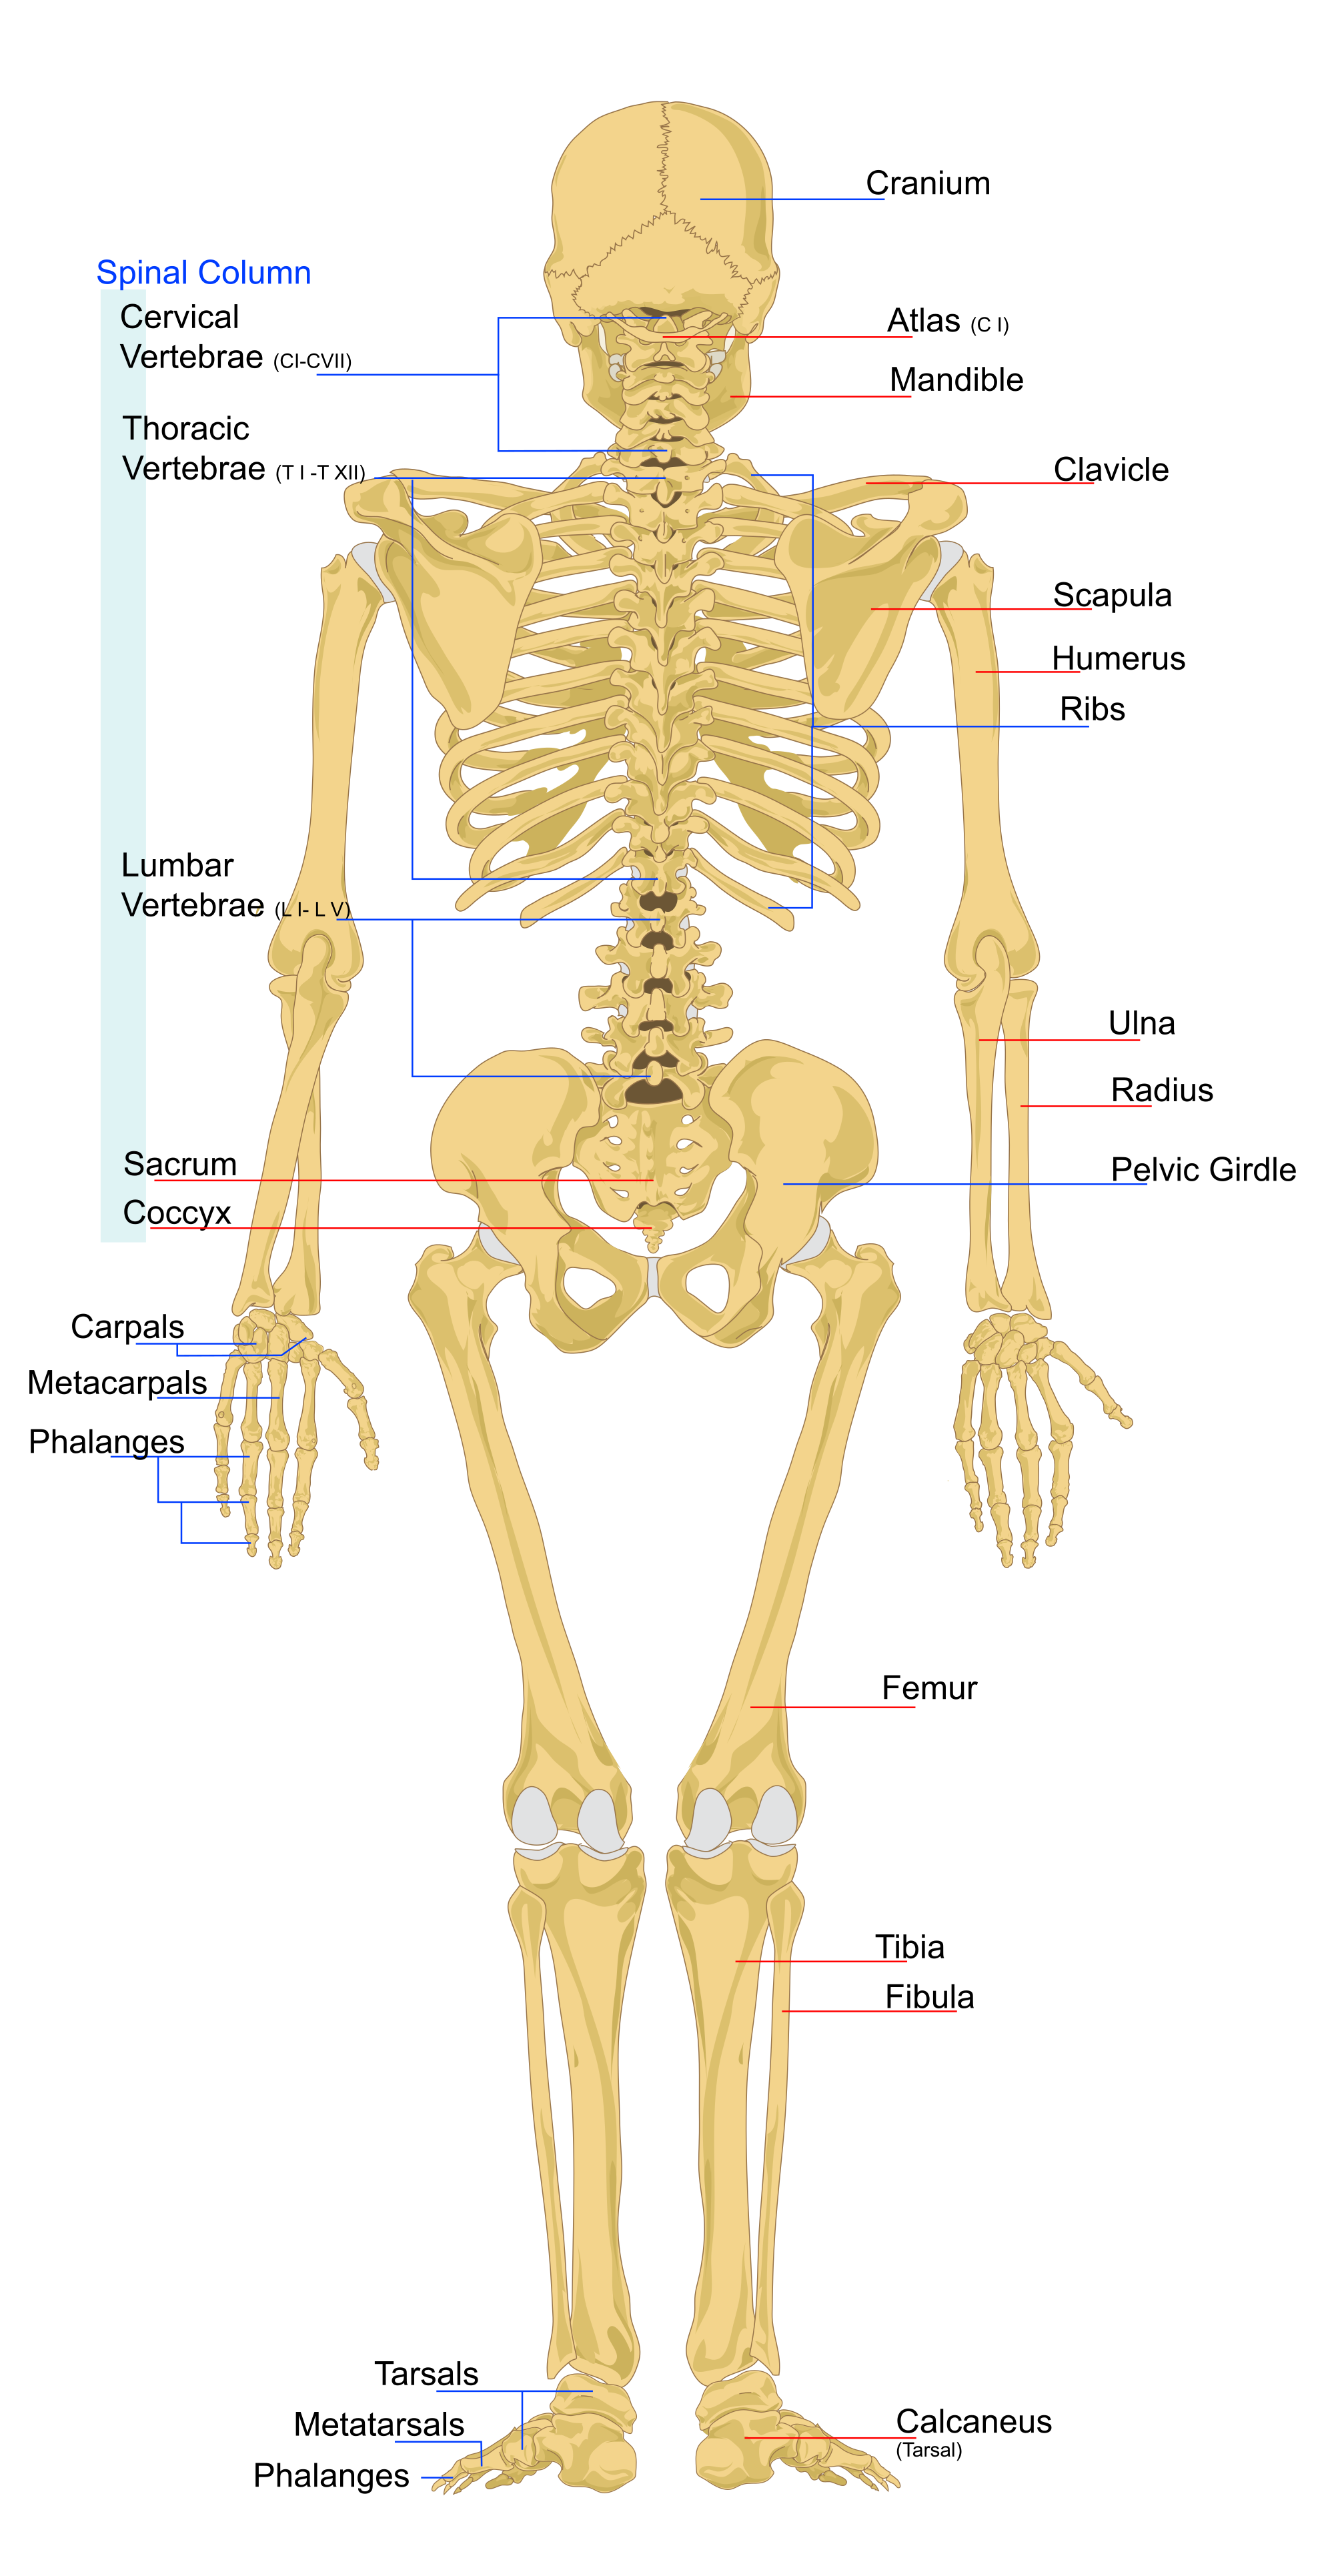
\includegraphics[width=0.7\linewidth]{./figures/locomotion/Human_skeleton_back_en} 

}

\caption{\href{https://commons.wikimedia.org/wiki/File:Human_skeleton_back_en.svg}{The human skeleton viewed from the back.}}\label{fig:humanskeletonback}
\end{figure}

The human skeleton takes 20 years before it is fully developed, and the bones contain marrow, which produces blood cells.

There exist several general differences between the male and female skeletons. The male skeleton, for example, is generally larger and heavier than the female skeleton. In the female skeleton, the bones of the skull are generally less angular. The female skeleton also has wider and shorter breastbone and slimmer wrists. There exist significant differences between the male and female pelvis which are related to the female's pregnancy and childbirth capabilities. The female pelvis is wider and shallower than the male pelvis. Female pelvises also have an enlarged pelvic outlet and a wider and more circular pelvic inlet. The angle between the pubic bones is known to be sharper in males, which results in a more circular, narrower, and near heart-shaped pelvis.

\hypertarget{the-axial-skeleton}{%
\subsection{The Axial Skeleton}\label{the-axial-skeleton}}

The axial skeleton (80 bones) is formed by the vertebral column (32 bones), a part of the rib cage (12 pairs of ribs and the sternum), and the skull (22 bones and 7 associated bones).



\begin{figure}

{\centering 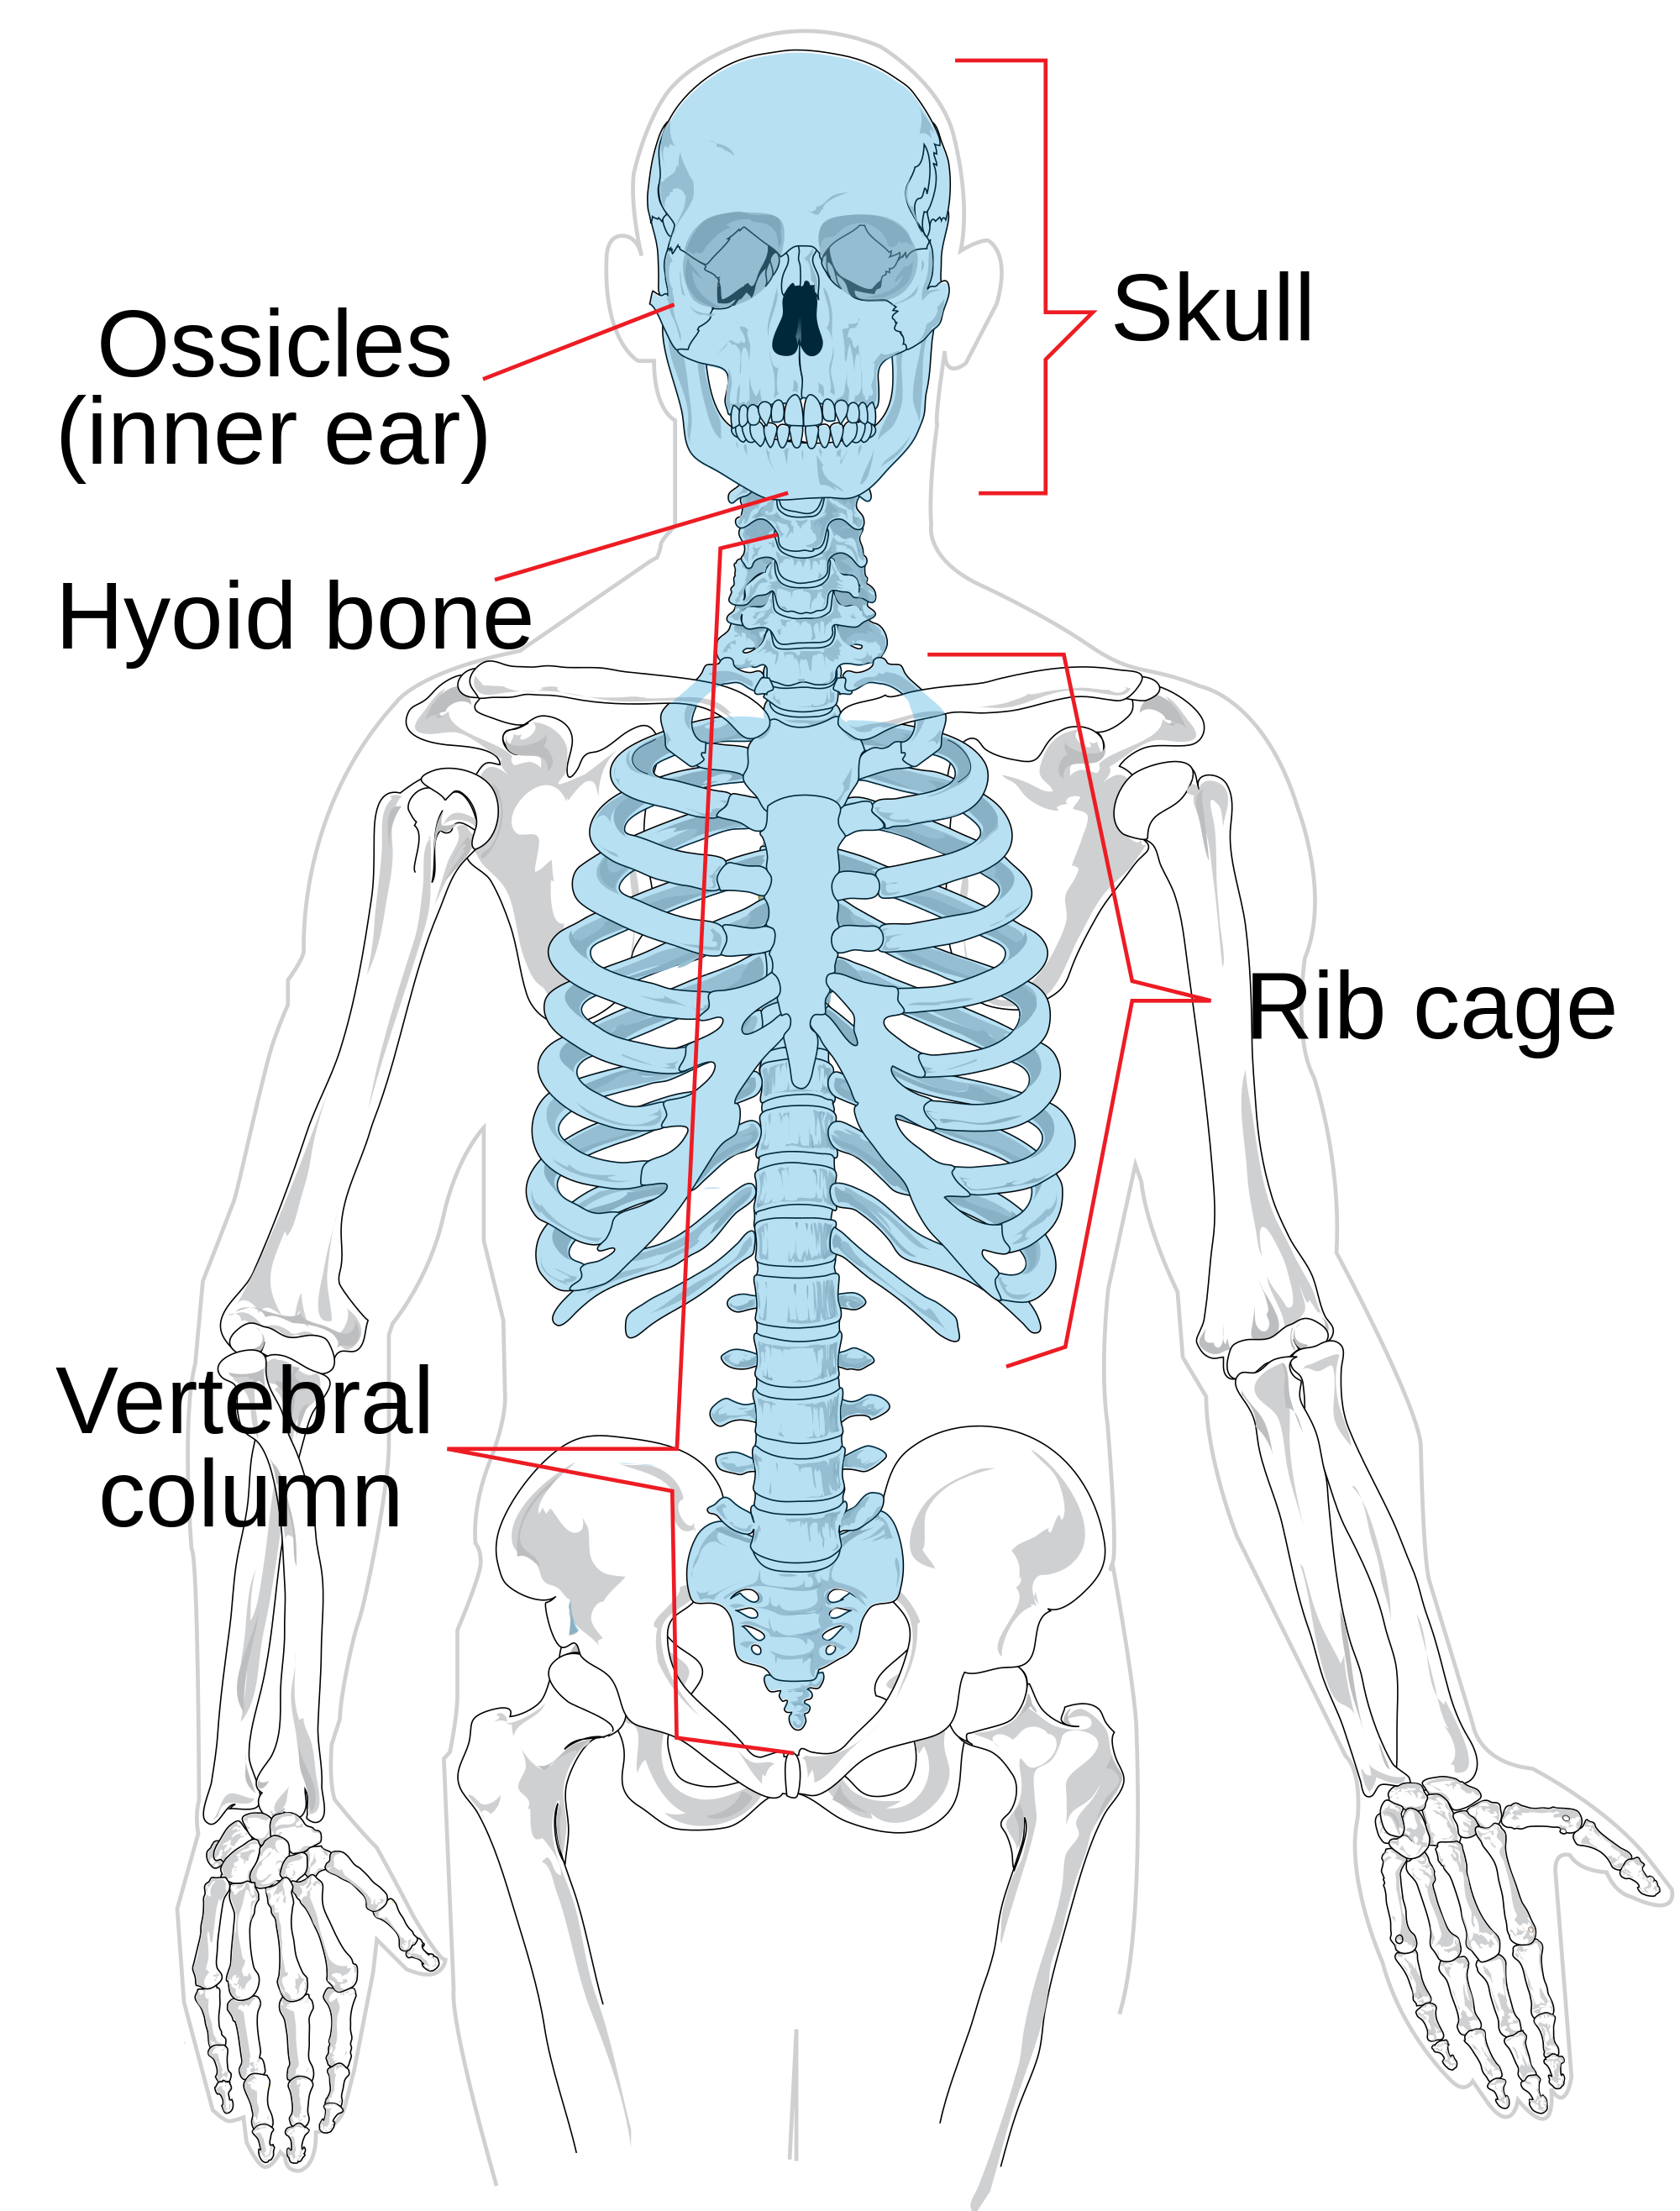
\includegraphics[width=0.7\linewidth]{./figures/locomotion/Axial_skeleton_diagram} 

}

\caption{\href{https://commons.wikimedia.org/wiki/File:Axial_skeleton_diagram.svg}{The Axial skeleton} consists of the bones in the head and trunk of the human body. It is composed of five parts; the human skull, the ossicles of the inner ear, the hyoid bone of the throat, the chest, and the vertebral column. The axial skeleton and the appendicular skeleton together form the complete skeleton.}\label{fig:axialskeleton}
\end{figure}

The upright posture of humans is maintained by the axial skeleton, which transmits the weight from the head, the trunk, and the upper extremities down to the lower extremities at the hip joints. The bones of the spine are supported by many ligaments. The erector spinae muscles are also supporting and are useful for balance.

\hypertarget{the-appendicular-skeleton}{%
\subsection{The Appendicular Skeleton}\label{the-appendicular-skeleton}}

The appendicular skeleton (126 bones) is formed by the pectoral girdles, the upper limbs, the pelvic girdle or pelvis, and the lower limbs. Their functions are to make locomotion possible and to protect the major organs of digestion, excretion and reproduction.



\begin{figure}

{\centering 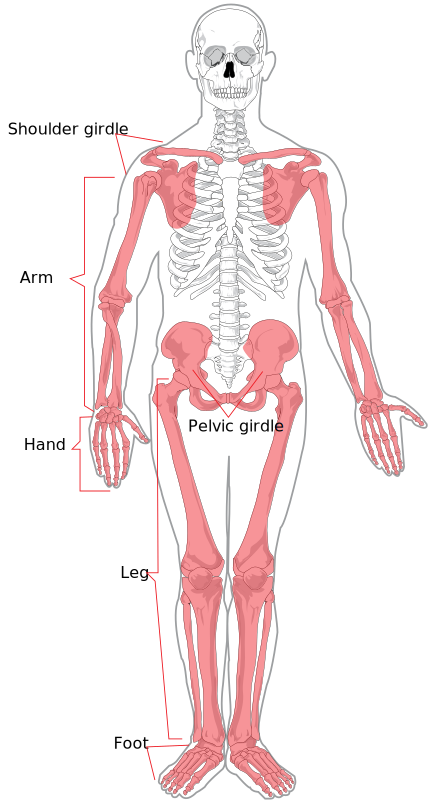
\includegraphics[width=0.7\linewidth]{./figures/locomotion/Appendicular_skeleton_diagram} 

}

\caption{\href{https://commons.wikimedia.org/wiki/File:Appendicular_skeleton_diagram.svg}{The appendicular skeleton (red) and the axial skeleton together form the complete skeleton.}}\label{fig:appendicularskeleton}
\end{figure}

\hypertarget{bone}{%
\subsection{Bone}\label{bone}}

A bone is a rigid organ that constitutes part of the vertebrate skeleton in animals. Bones protect the various organs of the body, produce red and white blood cells, store minerals, provide structure and support for the body, and enable mobility. Bones come in a variety of shapes and sizes and have a complex internal and external structure. They are lightweight yet strong and hard, and serve multiple functions.



\begin{figure}

{\centering 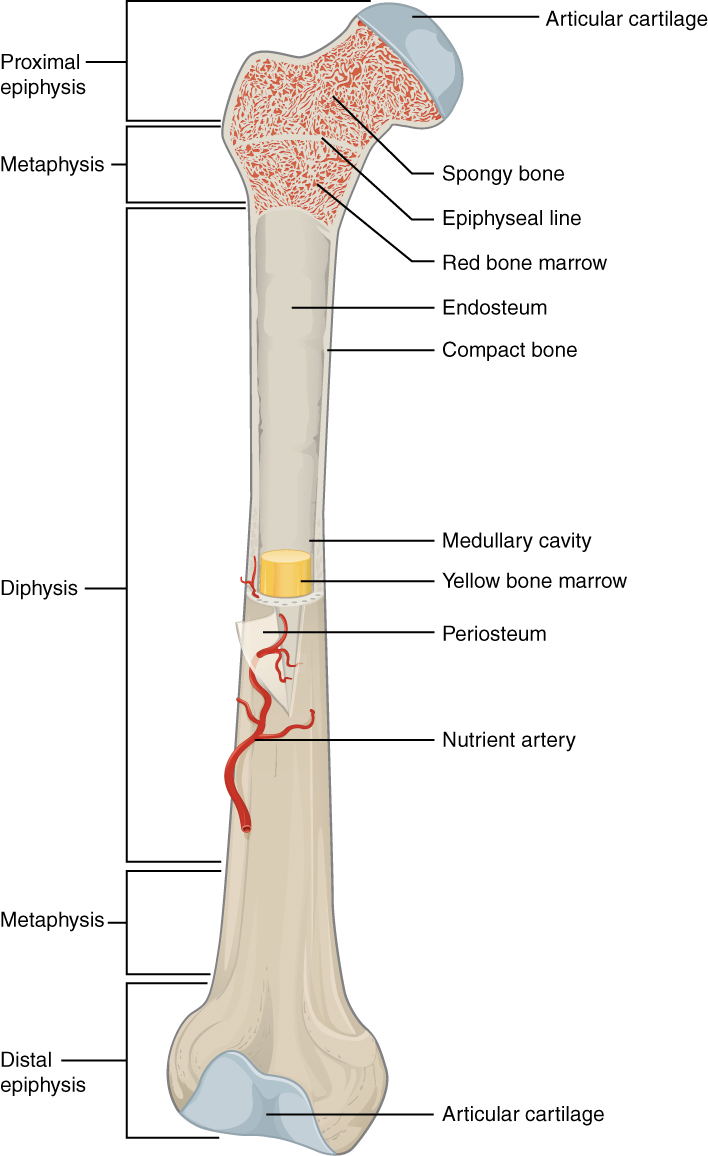
\includegraphics[width=0.7\linewidth]{./figures/locomotion/603_Anatomy_of_Long_Bone} 

}

\caption{\href{https://commons.wikimedia.org/wiki/File:603_Anatomy_of_Long_Bone.jpg}{Structure of a long bone.}}\label{fig:longbone}
\end{figure}



\begin{figure}

{\centering 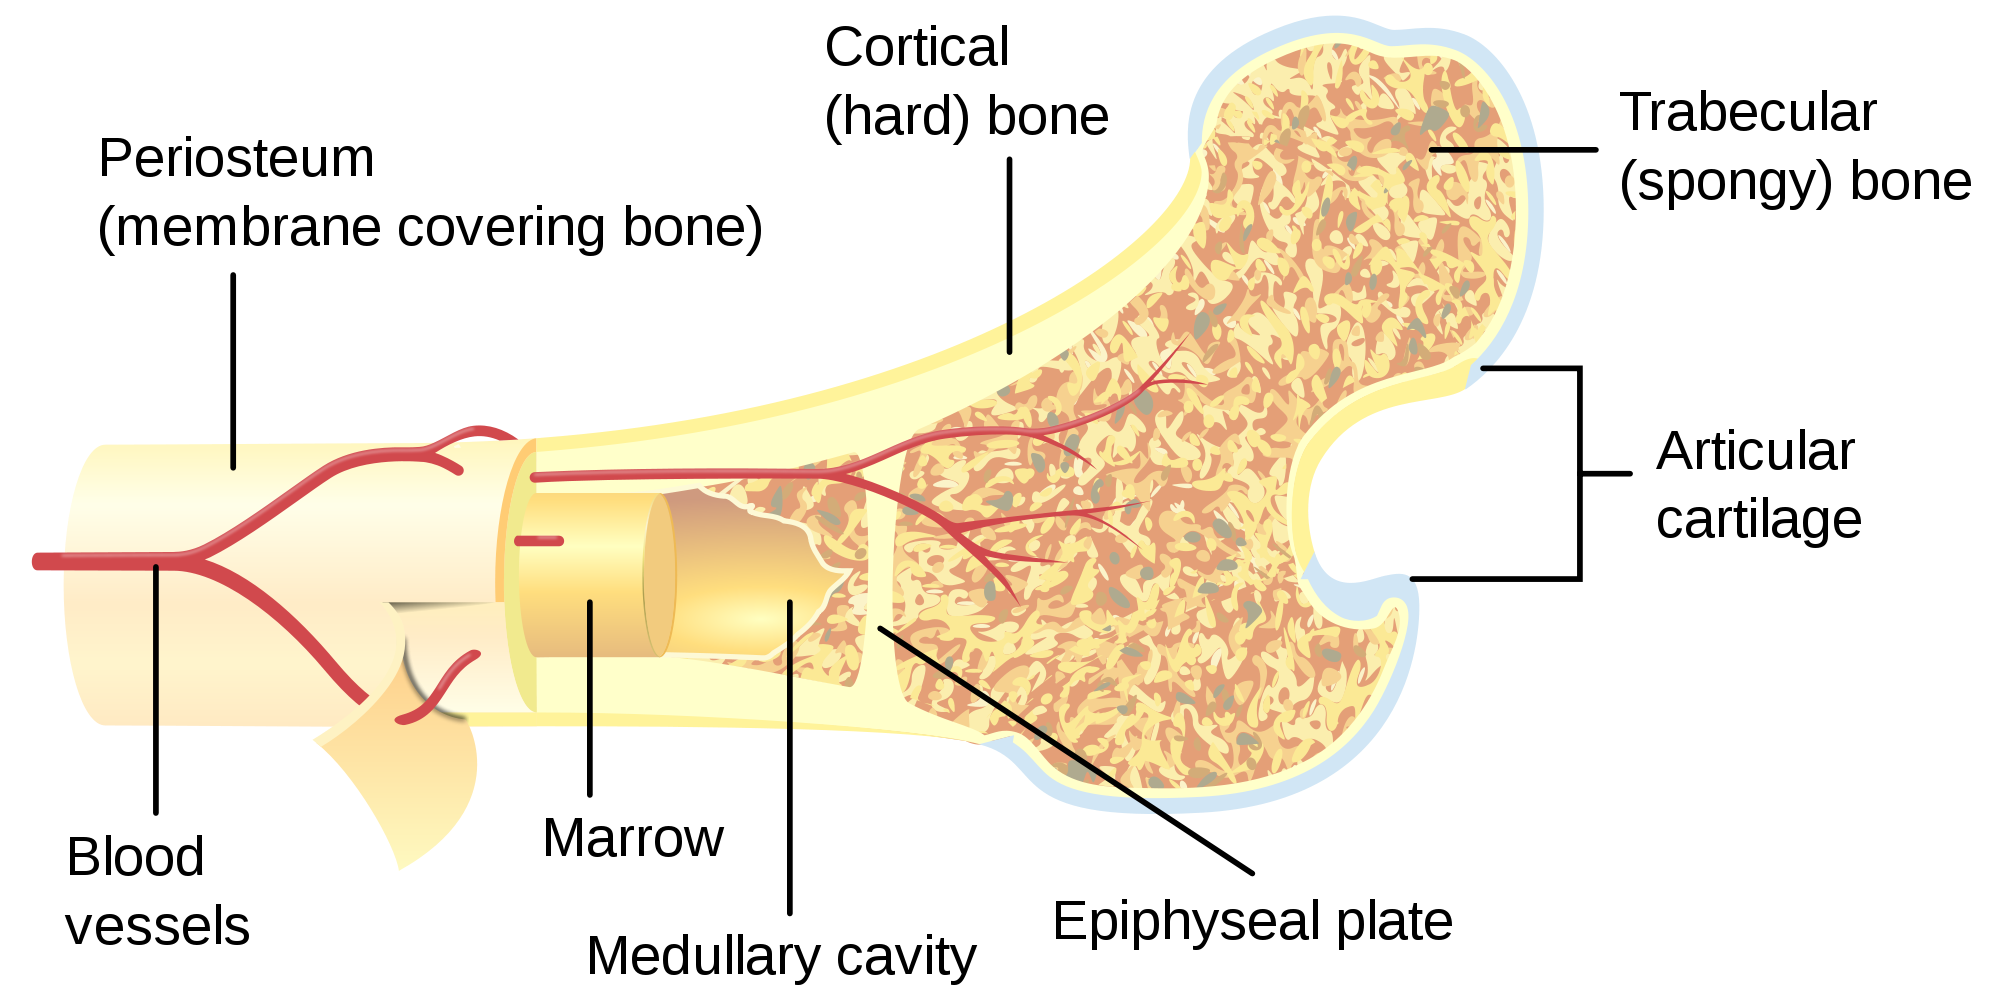
\includegraphics[width=0.7\linewidth]{./figures/locomotion/Bone_cross-section} 

}

\caption{\href{https://commons.wikimedia.org/wiki/File:Human_skeleton_back_en.svg}{Cross-section of human bone.}}\label{fig:bonecrossection}
\end{figure}

Bone tissue (osseous tissue) is a hard tissue, a type of dense connective tissue. It has a honeycomb-like matrix internally, which helps to give the bone rigidity. Bone tissue is made up of different types of bone cells. Osteoblasts and osteocytes are involved in the formation and mineralization of bone; osteoclasts are involved in the resorption of bone tissue. Modified (flattened) osteoblasts become the lining cells that form a protective layer on the bone surface. The mineralised matrix of bone tissue has an organic component of mainly collagen called ossein and an inorganic component of bone mineral made up of various salts. Bone tissue is a mineralized tissue of two types, cortical bone and cancellous bone. Other types of tissue found in bones include bone marrow, endosteum, periosteum, nerves, blood vessels and cartilage.



\begin{figure}

{\centering 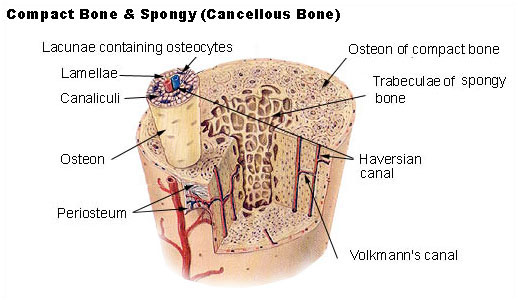
\includegraphics[width=0.7\linewidth]{./figures/locomotion/Illu_compact_spongy_bone} 

}

\caption{\href{https://commons.wikimedia.org/wiki/File:Illu_compact_spongy_bone.jpg}{A cross section of a long bone, showing the internal structure.}}\label{fig:anotherbonecrossection}
\end{figure}

The Greek word for bone is ὀστέον (``osteon''), hence the many terms that use it as a prefix---such as osteopathy.

Bone is not uniformly solid, but consists of a flexible matrix (about 30\%) and bound minerals (about 70\%) which are intricately woven and endlessly remodeled by a group of specialized bone cells. Their unique composition and design allows bones to be relatively hard and strong, while remaining lightweight.

Bone matrix is 90 to 95\% composed of elastic collagen fibers, also known as ossein, and the remainder is ground substance. The elasticity of collagen improves fracture resistance. The matrix is hardened by the binding of inorganic mineral salt, calcium phosphate, in a chemical arrangement known as calcium hydroxylapatite. It is the bone mineralization that give bones rigidity.

Bone is actively constructed and remodeled throughout life by special bone cells known as osteoblasts and osteoclasts. Within any single bone, the tissue is woven into two main patterns, known as cortical and cancellous bone, and each with different appearance and characteristics.

\hypertarget{cortical-bone}{%
\subsection{Cortical Bone}\label{cortical-bone}}

The hard outer layer of bones is composed of cortical bone, which is also called compact bone as it is much denser than cancellous bone. It forms the hard exterior (cortex) of bones. The cortical bone gives bone its smooth, white, and solid appearance, and accounts for 80\% of the total bone mass of an adult human skeleton. It facilitates bone's main functions - to support the whole body, to protect organs, to provide levers for movement, and to store and release chemical elements, mainly calcium. It consists of multiple microscopic columns, each called an osteon or Haversian system. Each column is multiple layers of osteoblasts and osteocytes around a central canal called the haversian canal. Volkmann's canals at right angles connect the osteons together. The columns are metabolically active, and as bone is reabsorbed and created the nature and location of the cells within the osteon will change. Cortical bone is covered by a periosteum on its outer surface, and an endosteum on its inner surface. The endosteum is the boundary between the cortical bone and the cancellous bone. The primary anatomical and functional unit of cortical bone is the osteon.

\hypertarget{cancellous-bone}{%
\subsection{Cancellous Bone}\label{cancellous-bone}}

Cancellous bone, also called trabecular or spongy bone, is the internal tissue of the skeletal bone and is an open cell porous network. Cancellous bone has a higher surface-area-to-volume ratio than cortical bone and it is less dense. This makes it weaker and more flexible. The greater surface area also makes it suitable for metabolic activities such as the exchange of calcium ions. Cancellous bone is typically found at the ends of long bones, near joints and in the interior of vertebrae. Cancellous bone is highly vascular and often contains red bone marrow where hematopoiesis, the production of blood cells, occurs. The primary anatomical and functional unit of cancellous bone is the trabecula. The trabeculae are aligned towards the mechanical load distribution that a bone experiences within long bones such as the femur. As far as short bones are concerned, trabecular alignment has been studied in the vertebral pedicle. Thin formations of osteoblasts covered in endosteum create an irregular network of spaces, known as trabeculae. Within these spaces are bone marrow and hematopoietic stem cells that give rise to platelets, red blood cells and white blood cells. Trabecular marrow is composed of a network of rod- and plate-like elements that make the overall organ lighter and allow room for blood vessels and marrow. Trabecular bone accounts for the remaining 20\% of total bone mass but has nearly ten times the surface area of compact bone.

The words cancellous and trabecular refer to the tiny lattice-shaped units (trabeculae) that form the tissue. It was first illustrated accurately in the engravings of Crisóstomo Martinez.

\hypertarget{the-bone-marrow-1}{%
\subsection{The Bone Marrow}\label{the-bone-marrow-1}}

Bone marrow, also known as myeloid tissue in red bone marrow, can be found in almost any bone that holds cancellous tissue. In newborns, all such bones are filled exclusively with red marrow or hematopoietic marrow, but as the child ages the hematopoietic fraction decreases in quantity and the fatty/ yellow fraction called marrow adipose tissue (MAT) increases in quantity. In adults, red marrow is mostly found in the bone marrow of the femur, the ribs, the vertebrae and pelvic bones.

\hypertarget{bone-cells}{%
\subsection{Bone cells}\label{bone-cells}}

Bone is a metabolically active tissue composed of several types of cells. These cells include osteoblasts, which are involved in the creation and mineralization of bone tissue, osteocytes, and osteoclasts, which are involved in the reabsorption of bone tissue. Osteoblasts and osteocytes are derived from osteoprogenitor cells, but osteoclasts are derived from the same cells that differentiate to form macrophages and monocytes. Within the marrow of the bone there are also hematopoietic stem cells. These cells give rise to other cells, including white blood cells, red blood cells, and platelets.



\begin{figure}

{\centering 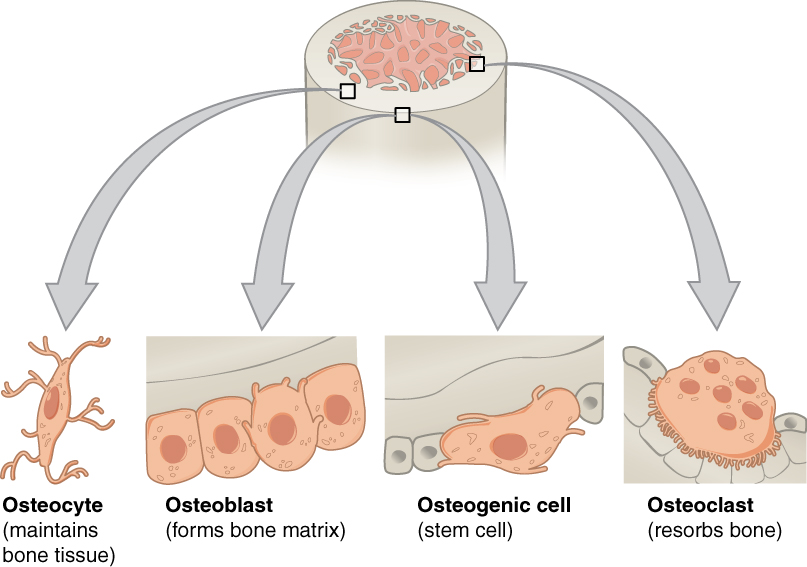
\includegraphics[width=0.7\linewidth]{./figures/locomotion/604_Bone_cells} 

}

\caption{\href{https://commons.wikimedia.org/wiki/File:604_Bone_cells.jpg}{Bone cells.}}\label{fig:bonecells}
\end{figure}

\hypertarget{osteoblast}{%
\subsection{Osteoblast}\label{osteoblast}}

Osteoblasts are mononucleate bone-forming cells. They are located on the surface of osteon seams and make a protein mixture known as osteoid, which mineralizes to become bone. The osteoid seam is a narrow region of newly formed organic matrix, not yet mineralized, located on the surface of a bone. Osteoid is primarily composed of Type I collagen. Osteoblasts also manufacture hormones, such as prostaglandins, to act on the bone itself. The osteoblast creates and repairs new bone by actually building around itself. First, the osteoblast puts up collagen fibers. These collagen fibers are used as a framework for the osteoblasts' work. The osteoblast then deposits calcium phosphate which is hardened by hydroxide and bicarbonate ions. The brand new bone created by the osteoblast is called osteoid. Once the osteoblast is finished working it is actually trapped inside the bone once it hardens. When the osteoblast becomes trapped, it becomes known as an osteocyte. Other osteoblasts remain on the top of the new bone and are used to protect the underlying bone, these become known as lining cells.

\hypertarget{osteocyte}{%
\subsection{Osteocyte}\label{osteocyte}}

Osteocytes are mostly inactive osteoblasts. Osteocytes originate from osteoblasts that have migrated into and become trapped and surrounded by bone matrix that they themselves produced. The spaces they occupy are known as lacunae. Osteocytes have many processes that reach out to meet osteoblasts and other osteocytes probably for the purposes of communication. Osteocytes remain in contact with other cells in the bone through gap junctions---coupled cell processes---which pass through small channels in the bone matrix called the canaliculi.

\hypertarget{osteoclast}{%
\subsection{Osteoclast}\label{osteoclast}}

Osteoclasts are very large multinucleate cells that are responsible for the breakdown of bones by the process of bone resorption. New bone is then formed by the osteoblasts. Bone is constantly remodelled by the resorption of osteoclasts and created by osteoblasts. Osteoclasts are large cells with multiple nuclei located on bone surfaces in what are called Howship's lacunae (or resorption pits). These lacunae are the result of surrounding bone tissue that has been reabsorbed. Because the osteoclasts are derived from a monocyte stem-cell lineage, they are equipped with phagocytic-like mechanisms similar to circulating macrophages. Osteoclasts mature and/or migrate to discrete bone surfaces. Upon arrival, active enzymes, such as tartrate resistant acid phosphatase, are secreted against the mineral substrate.{[}citation needed{]} The reabsorption of bone by osteoclasts also plays a role in calcium homeostasis.

\hypertarget{extracellular-matrix}{%
\subsection{Extracellular Matrix}\label{extracellular-matrix}}

Bones consist of living cells embedded in a mineralized organic matrix. This matrix consists of organic components, mainly type I collagen -- ``organic'' referring to materials produced as a result of the human body -- and inorganic components, primarily hydroxyapatite and other salts of calcium and phosphate. Above 30\% of the acellular part of bone consists of the organic components, and 70\% of salts. The collagen fibers give bone its tensile strength, and the interspersed crystals of hydroxyapatite give bone its compressive strength. These effects are synergistic.

The inorganic composition of bone (bone mineral) is primarily formed from salts of calcium and phosphate, the major salt being hydroxyapatite (Ca10(PO4)6(OH)2). The exact composition of the matrix may be subject to change over time due to nutrition and biomineralization, with the ratio of calcium to phosphate varying between 1.3 and 2.0 (per weight), and trace minerals such as magnesium, sodium, potassium and carbonate also being found.

\hypertarget{the-muscular-system}{%
\section{The Muscular System}\label{the-muscular-system}}

The muscular system is an organ system consisting of skeletal, smooth and cardiac muscles. It permits movement of the body, maintains posture and circulates blood throughout the body. The muscular systems in vertebrates are controlled through the nervous system although some muscles (such as the cardiac muscle) can be completely autonomous. Together with the skeletal system, it forms the musculoskeletal system, which is responsible for movement of the human body.

There are three distinct types of muscles:

\begin{itemize}
\tightlist
\item
  Skeletal muscle or ``voluntary muscle'' is anchored by tendons (or by aponeuroses at a few places) to bone and is used to effect skeletal movement such as locomotion and in maintaining posture. Though this postural control is generally maintained as an unconscious reflex, the muscles responsible react to conscious control like non-postural muscles. An average adult male is made up of 42\% of skeletal muscle and an average adult female is made up of 36\% (as a percentage of body mass).
\item
  Smooth muscle or ``involuntary muscle'' is found within the walls of organs and structures such as the esophagus, stomach, intestines, bronchi, uterus, urethra, bladder, blood vessels, and the arrector pili in the skin (in which it controls erection of body hair). Unlike skeletal muscle, smooth muscle is not under conscious control.
\item
  Cardiac muscle (myocardium), is also an ``involuntary muscle'' but is more akin in structure to skeletal muscle, and is found only in the heart.
\end{itemize}



Skeletal muscle is arranged in discrete muscles, an example of which is the biceps brachii (biceps). The tough, fibrous epimysium of skeletal muscle is both connected to and continuous with the tendons. In turn, the tendons connect to the periosteum layer surrounding the bones, permitting the transfer of force from the muscles to the skeleton. Together, these fibrous layers, along with tendons and ligaments, constitute the deep fascia of the body.

\begin{figure}

{\centering 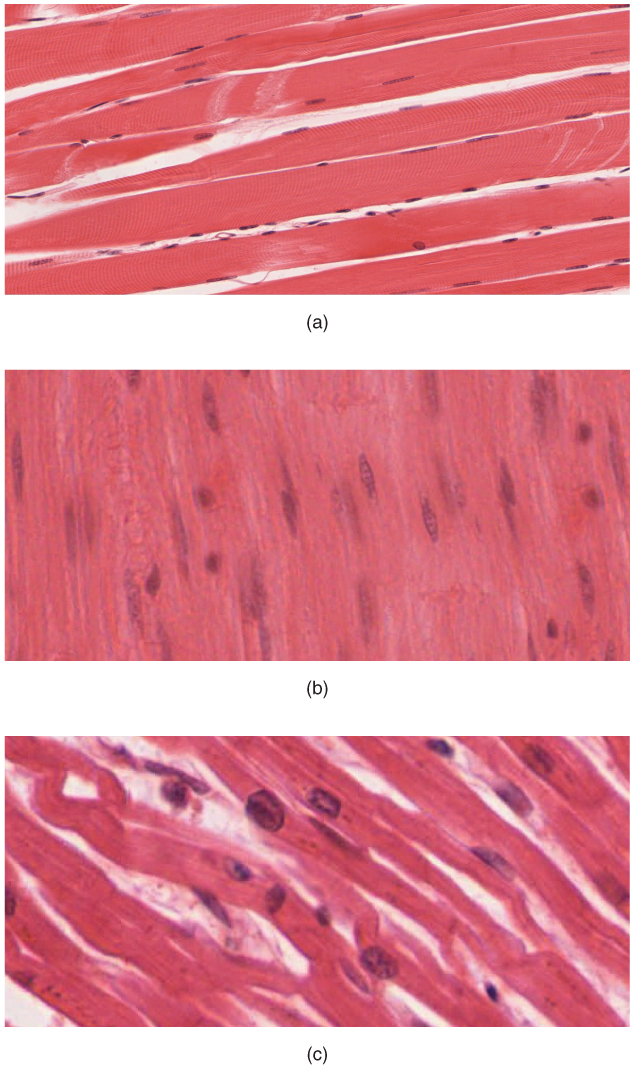
\includegraphics[width=0.7\linewidth]{./figures/locomotion/414_Skeletal_Smooth_Cardiac} 

}

\caption{\href{https://upload.wikimedia.org/wikipedia/commons/e/e5/414_Skeletal_Smooth_Cardiac.jpg}{The body contains three types of muscle tissue}: (a) skeletal muscle, (b) smooth muscle, and (c) cardiac muscle.}\label{fig:threetypesofmuscle}
\end{figure}

Skeletal muscles, like other striated muscles, are composed of myocytes, or muscle fibers, which are in turn composed of myofibrils, which are composed of sarcomeres, the basic building block of striated muscle tissue. Upon stimulation by an action potential, skeletal muscles perform a coordinated contraction by shortening each sarcomere. The best proposed model for understanding contraction is the sliding filament model of muscle contraction. Within the sarcomere, actin and myosin fibers overlap in a contractile motion towards each other. Myosin filaments have club-shaped heads that project toward the actin filaments.



\begin{figure}

{\centering 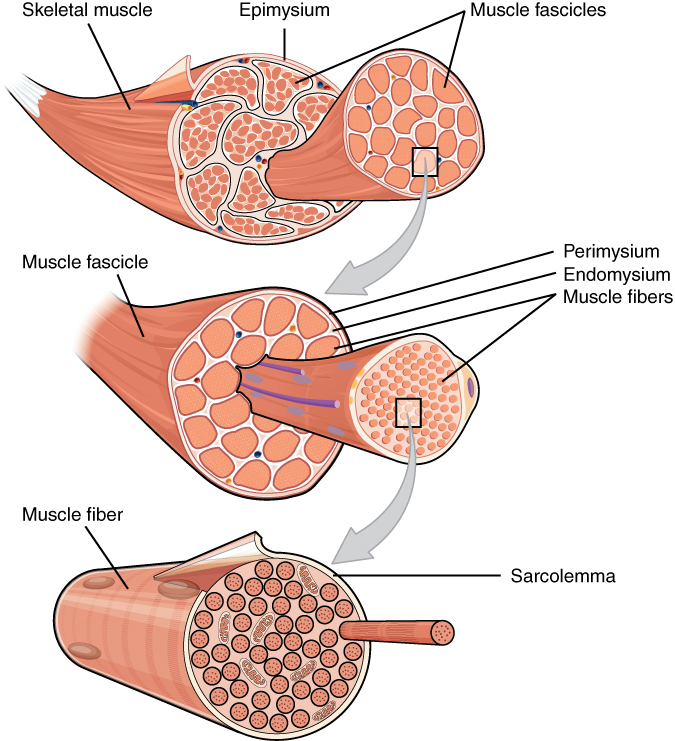
\includegraphics[width=0.7\linewidth]{./figures/locomotion/1007_Muscle_Fibes_(large)} 

}

\caption{\href{https://upload.wikimedia.org/wikipedia/commons/d/dd/1007_Muscle_Fibes_\%28large\%29.jpg}{Bundles of muscle fibers, called fascicles, are covered by the perimysium. Muscle fibers are covered by the endomysium.}}\label{fig:skeletalmuscle}
\end{figure}



\begin{figure}

{\centering 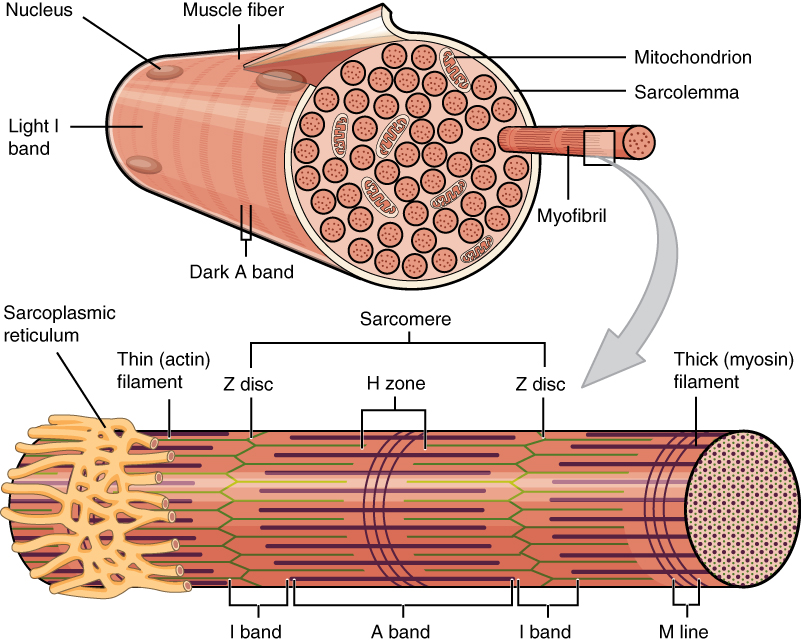
\includegraphics[width=0.7\linewidth]{./figures/locomotion/1022_Muscle_Fibers_(small)} 

}

\caption{\href{https://commons.wikimedia.org/wiki/File:1022_Muscle_Fibers_(small).jpg}{A skeletal muscle fiber is surrounded by a plasma membrane called the sarcolemma, which contains sarcoplasm, the cytoplasm of muscle cells. A muscle fiber is composed of many fibrils, which give the cell its striated appearance.}}\label{fig:musclefibre}
\end{figure}

Larger structures along the myosin filament called myosin heads are used to provide attachment points on binding sites for the actin filaments. The myosin heads move in a coordinated style; they swivel toward the center of the sarcomere, detach and then reattach to the nearest active site of the actin filament. This is called a ratchet type drive system.

This process consumes large amounts of adenosine triphosphate (ATP), the energy source of the cell. ATP binds to the cross bridges between myosin heads and actin filaments. The release of energy powers the swiveling of the myosin head. When ATP is used, it becomes adenosine diphosphate (ADP), and since muscles store little ATP, they must continuously replace the discharged ADP with ATP. Muscle tissue also contains a stored supply of a fast acting recharge chemical, creatine phosphate, which when necessary can assist with the rapid regeneration of ADP into ATP.

Calcium ions are required for each cycle of the sarcomere. Calcium is released from the sarcoplasmic reticulum into the sarcomere when a muscle is stimulated to contract. This calcium uncovers the actin binding sites. When the muscle no longer needs to contract, the calcium ions are pumped from the sarcomere and back into storage in the sarcoplasmic reticulum.

There are approximately 639 skeletal muscles in the human body.



\begin{figure}

{\centering 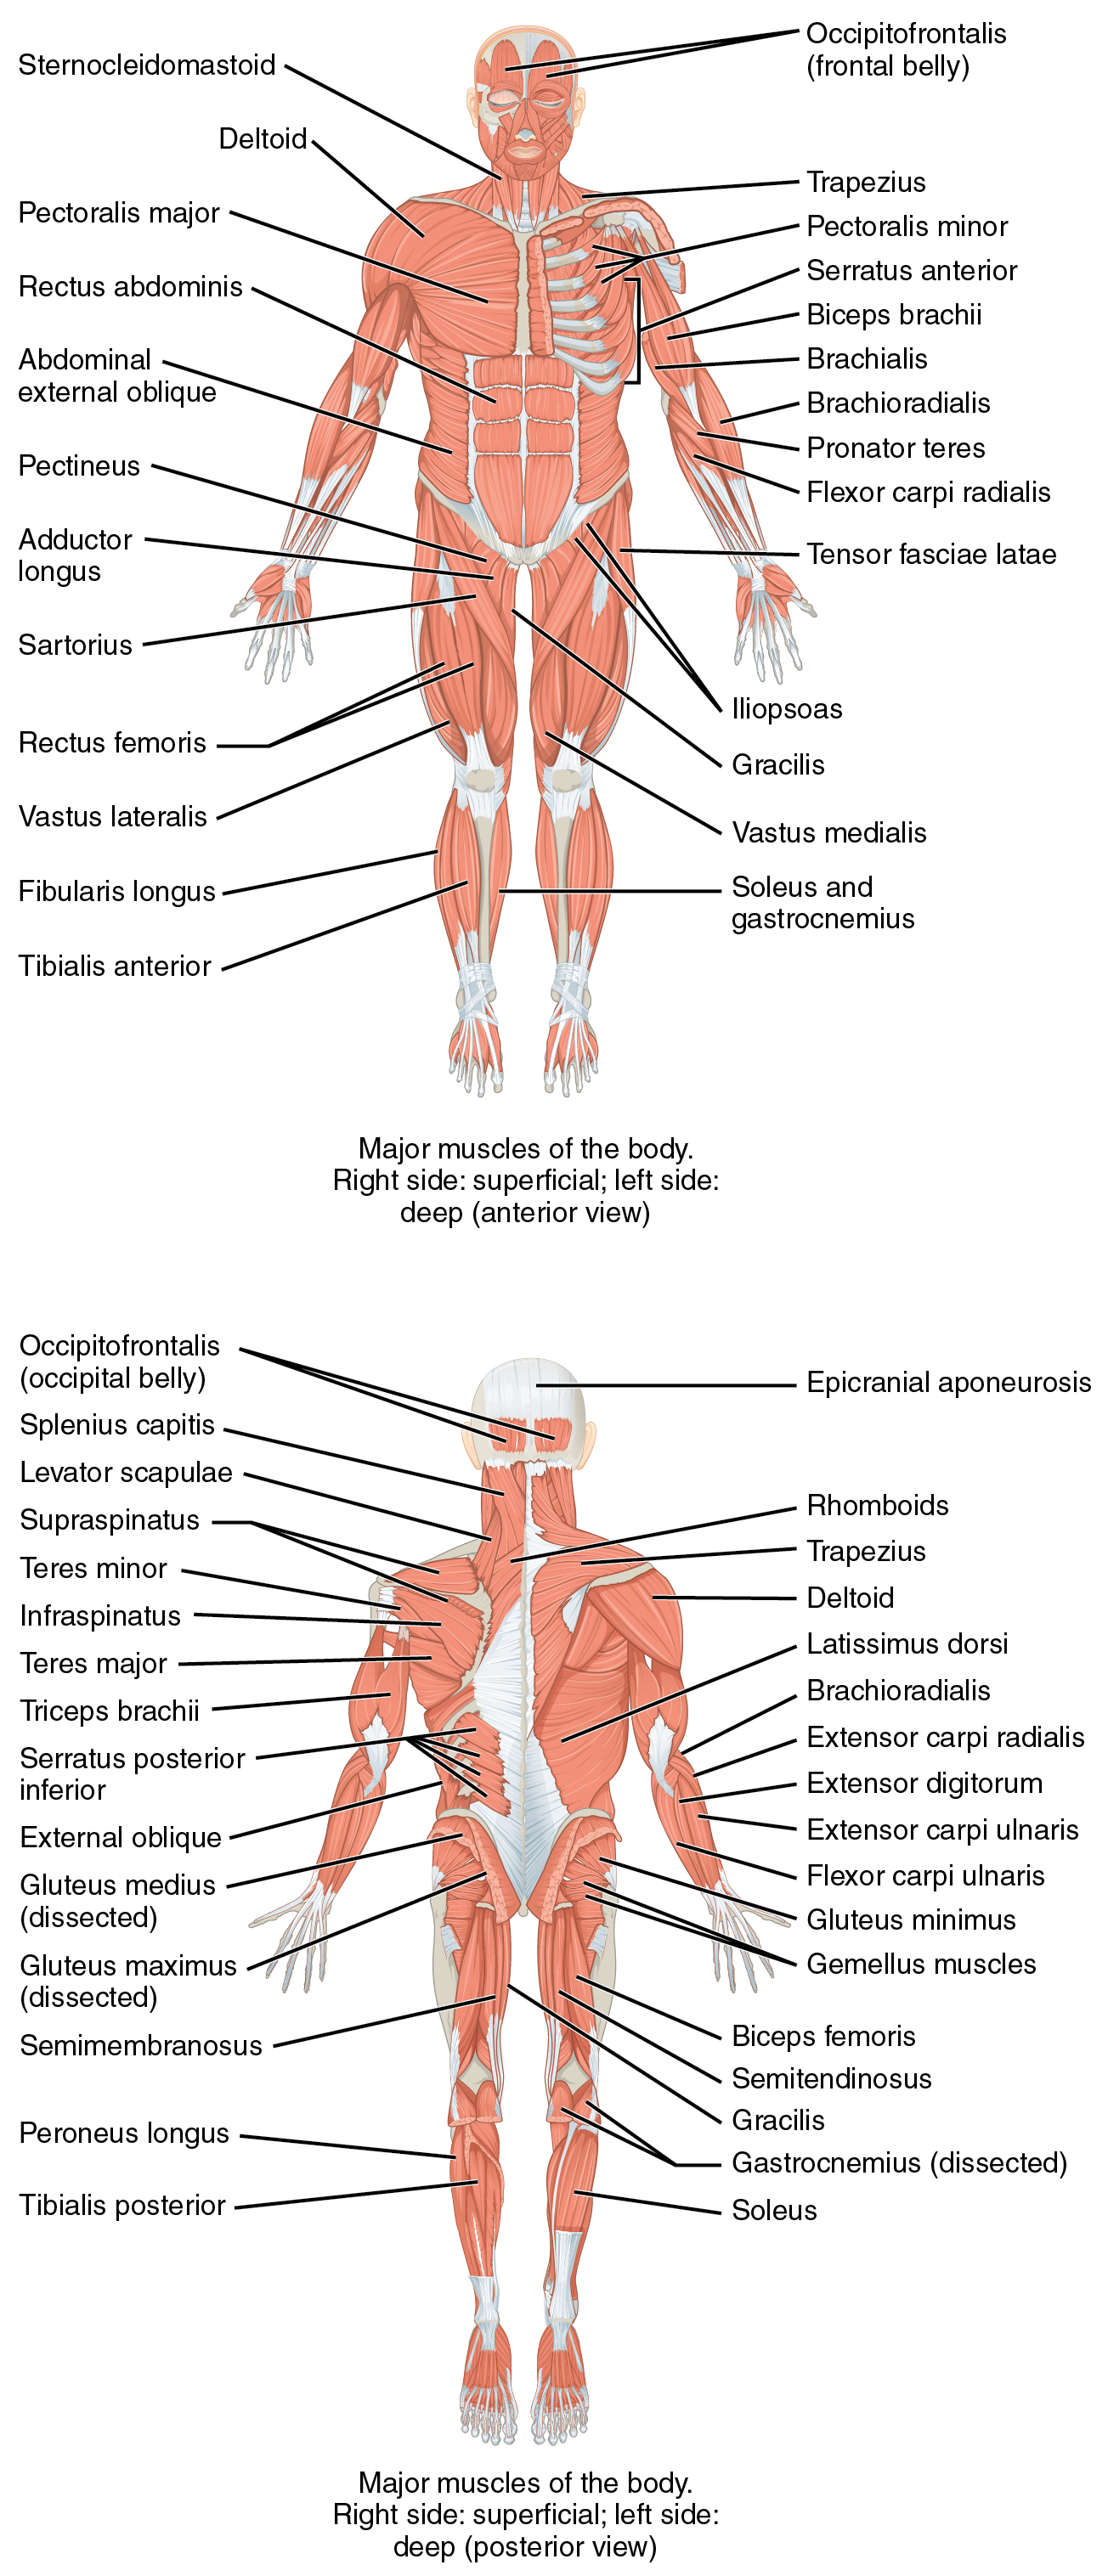
\includegraphics[width=0.7\linewidth]{./figures/locomotion/1105_Anterior_and_Posterior_Views_of_Muscles} 

}

\caption{\href{https://commons.wikimedia.org/wiki/File:1105_Anterior_and_Posterior_Views_of_Muscles.jpg}{On the anterior and posterior views of the muscular system above, superficial muscles (those at the surface) are shown on the right side of the body while deep muscles (those underneath the superficial muscles) are shown on the left half of the body. For the legs, superficial muscles are shown in the anterior view while the posterior view shows both superficial and deep muscles.}}\label{fig:muscularsystem}
\end{figure}

Heart muscles are distinct from skeletal muscles because the muscle fibers are laterally connected to each other. Furthermore, just as with smooth muscles, their movement is involuntary. Heart muscles are controlled by the sinus node influenced by the autonomic nervous system.

Smooth muscles are controlled directly by the autonomic nervous system and are involuntary, meaning that they are incapable of being moved by conscious thought. Functions such as heartbeat and lungs (which are capable of being willingly controlled, be it to a limited extent) are involuntary muscles but are not smooth muscles.

\hypertarget{muscle-contraction}{%
\subsection{Muscle Contraction}\label{muscle-contraction}}

Muscle contraction is the activation of tension-generating sites within muscle fibers. In physiology, muscle contraction does not necessarily mean muscle shortening because muscle tension can be produced without changes in muscle length, such as when holding a heavy book or a dumbbell at the same position. The termination of muscle contraction is followed by muscle relaxation, which is a return of the muscle fibers to their low tension-generating state.

At rest, the body produces the majority of its ATP aerobically in the mitochondria without producing lactic acid or other fatiguing byproducts. During exercise, the method of ATP production varies depending on the fitness of the individual as well as the duration and intensity of exercise. At lower activity levels, when exercise continues for a long duration (several minutes or longer), energy is produced aerobically by combining oxygen with carbohydrates and fats stored in the body.

During activity that is higher in intensity, with possible duration decreasing as intensity increases, ATP production can switch to anaerobic pathways, such as the use of the creatine phosphate and the phosphagen system or anaerobic glycolysis. Aerobic ATP production is biochemically much slower and can only be used for long-duration, low-intensity exercise, but produces no fatiguing waste products that can not be removed immediately from the sarcomere and the body, and it results in a much greater number of ATP molecules per fat or carbohydrate molecule. Aerobic training allows the oxygen delivery system to be more efficient, allowing aerobic metabolism to begin quicker. Anaerobic ATP production produces ATP much faster and allows near-maximal intensity exercise, but also produces significant amounts of lactic acid which renders high-intensity exercise unsustainable for more than several minutes. The phosphagen system is also anaerobic. It allows for the highest levels of exercise intensity, but intramuscular stores of phosphocreatine are very limited and can only provide energy for exercises lasting up to ten seconds. Recovery is very quick, with full creatine stores regenerated within five minutes
Muscle contractions can be described based on two variables: length and tension. A muscle contraction is described as isometric if the muscle tension changes but the muscle length remains the same. In contrast, a muscle contraction is isotonic if muscle tension remains the same throughout the contraction. If the muscle length shortens, the contraction is concentric; if the muscle length lengthens, the contraction is eccentric. In natural movements that underlie locomotor activity, muscle contractions are multifaceted as they are able to produce changes in length and tension in a time-varying manner. Therefore, neither length nor tension is likely to remain the same in muscles that contract during locomotor activity.

In vertebrates, skeletal muscle contractions are neurogenic as they require synaptic input from motor neurons to produce muscle contractions. A single motor neuron is able to innervate multiple muscle fibers, thereby causing the fibers to contract at the same time. Once innervated, the protein filaments within each skeletal muscle fiber slide past each other to produce a contraction, which is explained by the sliding filament theory. The contraction produced can be described as a twitch, summation, or tetanus, depending on the frequency of action potentials. In skeletal muscles, muscle tension is at its greatest when the muscle is stretched to an intermediate length as described by the length-tension relationship.

Unlike skeletal muscle, the contractions of smooth and cardiac muscles are myogenic (meaning that they are initiated by the smooth or heart muscle cells themselves instead of being stimulated by an outside event such as nerve stimulation), although they can be modulated by stimuli from the autonomic nervous system. The mechanisms of contraction in these muscle tissues are similar to those in skeletal muscle tissues.

Muscle contractions can be described based on two variables: force and length. Force itself can be differentiated as either tension or load. Muscle tension is the force exerted by the muscle on an object whereas a load is the force exerted by an object on the muscle. When muscle tension changes without any corresponding changes in muscle length, the muscle contraction is described as isometric. If the muscle length changes while muscle tension remains the same, then the muscle contraction is isotonic. In an isotonic contraction, the muscle length can either shorten to produce a concentric contraction or lengthen to produce an eccentric contraction. In natural movements that underlie locomotor activity, muscle contractions are multifaceted as they are able to produce changes in length and tension in a time-varying manner. Therefore, neither length nor tension is likely to remain constant when the muscle is active during locomotor activity.

An isometric contraction of a muscle generates tension without changing length. An example can be found when the muscles of the hand and forearm grip an object; the joints of the hand do not move, but muscles generate sufficient force to prevent the object from being dropped.

In isotonic contraction, the tension in the muscle remains constant despite a change in muscle length. This occurs when a muscle's force of contraction matches the total load on the muscle.

\hypertarget{skeletal-muscle}{%
\subsection{Skeletal Muscle}\label{skeletal-muscle}}

Excluding reflexes, all skeletal muscles contractions occur as a result of conscious effort originating in the brain. The brain sends electrochemical signals through the nervous system to the motor neuron that innervates several muscle fibers. In the case of some reflexes, the signal to contract can originate in the spinal cord through a feedback loop with the grey matter. Other actions such as locomotion, breathing, and chewing have a reflex aspect to them: the contractions can be initiated both consciously or unconsciously.

A neuromuscular junction is a chemical synapse formed by the contact between a motor neuron and a muscle fiber. It is the site in which a motor neuron transmits a signal to a muscle fiber to initiate muscle contraction.



\begin{figure}

{\centering 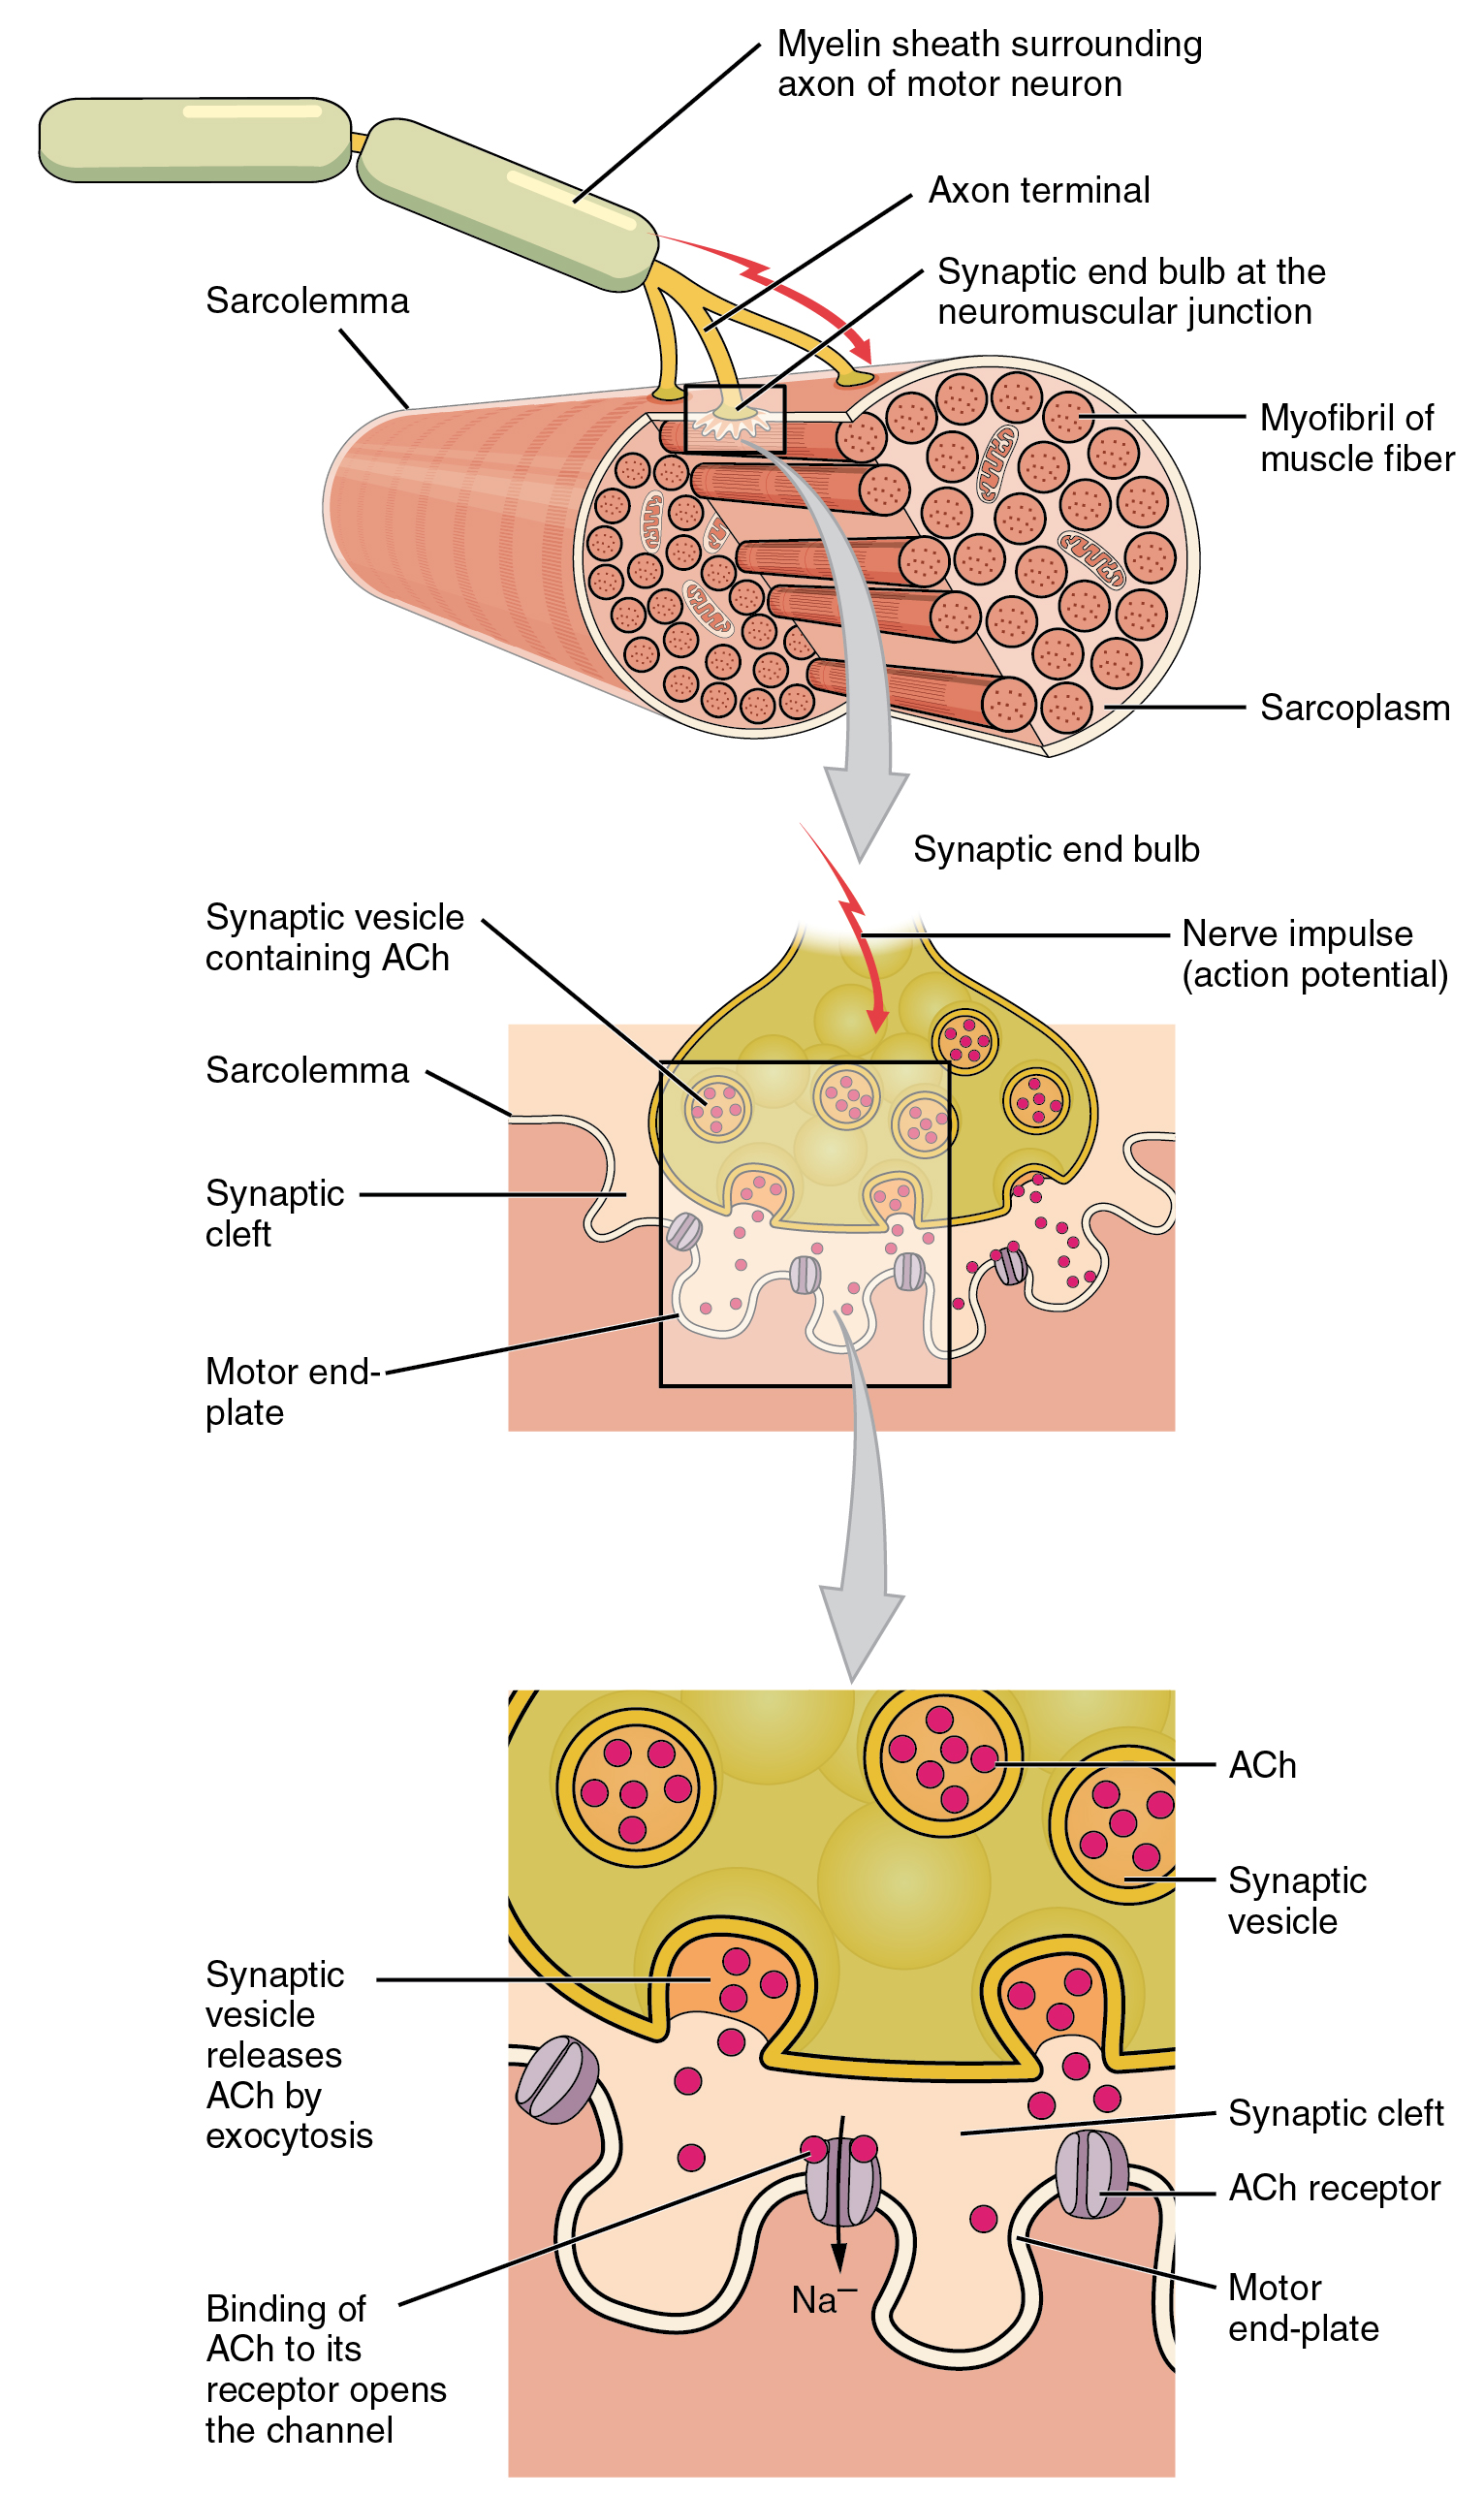
\includegraphics[width=0.7\linewidth]{./figures/locomotion/1009_Motor_End_Plate_and_Innervation} 

}

\caption{\href{https://upload.wikimedia.org/wikipedia/commons/5/57/1009_Motor_End_Plate_and_Innervation.jpg}{Structure of neuromuscular junction.}}\label{fig:neuromuscularjunction}
\end{figure}

The sequence of events that results in the depolarization of the muscle fiber at the neuromuscular junction begins when an action potential is initiated in the cell body of a motor neuron, which is then propagated by saltatory conduction along its axon toward the neuromuscular junction. Once it reaches the terminal bouton, the action potential causes a Ca\textsuperscript{2+} ion influx into the terminal by way of the voltage-gated calcium channels. The Ca\textsuperscript{2+} influx causes synaptic vesicles containing the neurotransmitter acetylcholine to fuse with the plasma membrane, releasing acetylcholine into the synaptic cleft between the motor neuron terminal and the neuromuscular junction of the skeletal muscle fiber. Acetylcholine diffuses across the synapse and binds to and activates nicotinic acetylcholine receptors on the neuromuscular junction. Activation of the nicotinic receptor opens its intrinsic sodium/potassium channel, causing sodium to rush in and potassium to trickle out. As a result, the sarcolemma reverses polarity and its voltage quickly jumps from the resting membrane potential of -90mV to as high as +75mV as sodium enters. The membrane potential then becomes hyperpolarized when potassium exits and is then adjusted back to the resting membrane potential. This rapid fluctuation is called the end-plate potential The voltage-gated ion channels of the sarcolemma next to the end plate open in response to the end plate potential. These voltage-gated channels are sodium and potassium specific and only allow one through. This wave of ion movements creates the action potential that spreads from the motor end plate in all directions. If action potentials stop arriving, then acetylcholine ceases to be released from the terminal bouton. The remaining acetylcholine in the synaptic cleft is either degraded by active acetylcholine esterase or reabsorbed by the synaptic knob and none is left to replace the degraded acetylcholine.

\hypertarget{excitation-contraction-coupling}{%
\subsection{Excitation-contraction Coupling}\label{excitation-contraction-coupling}}

Excitation--contraction coupling is the process by which a muscular action potential in the muscle fiber causes the myofibrils to contract. In skeletal muscle, excitation--contraction coupling relies on a direct coupling between key proteins, the sarcoplasmic reticulum (SR) calcium release channel (identified as the ryanodine receptor, RyR) and voltage-gated L-type calcium channels (identified as dihydropyridine receptors, DHPRs). DHPRs are located on the sarcolemma (which includes the surface sarcolemma and the transverse tubules), while the RyRs reside across the SR membrane. The close apposition of a transverse tubule and two SR regions containing RyRs is described as a triad and is predominantly where excitation--contraction coupling takes place. Excitation--contraction coupling occurs when depolarization of skeletal muscle cell results in a muscle action potential, which spreads across the cell surface and into the muscle fiber's network of T-tubules, thereby depolarizing the inner portion of the muscle fiber. Depolarization of the inner portions activates dihydropyridine receptors in the terminal cisternae, which are in close proximity to ryanodine receptors in the adjacent sarcoplasmic reticulum. The activated dihydropyridine receptors physically interact with ryanodine receptors to activate them via foot processes (involving conformational changes that allosterically activates the ryanodine receptors). As the ryanodine receptors open, Ca\textsuperscript{2+} is released from the sarcoplasmic reticulum into the local junctional space, which then diffuses into the bulk cytoplasm to cause a calcium spark. Note that the sarcoplasmic reticulum has a large calcium buffering capacity partially due to a calcium-binding protein called calsequestrin. The near synchronous activation of thousands of calcium sparks by the action potential causes a cell-wide increase in calcium giving rise to the upstroke of the calcium transient. The Ca\textsuperscript{2+} released into the cytosol binds to Troponin C by the actin filaments, to allow crossbridge cycling, producing force and, in some situations, motion. The sarco/endoplasmic reticulum calcium-ATPase (SERCA) actively pumps Ca\textsuperscript{2+} back into the sarcoplasmic reticulum. As Ca\textsuperscript{2+} declines back to resting levels, the force declines and relaxation occurs.

\hypertarget{the-sliding-filament-theory}{%
\subsection{The Sliding Filament Theory}\label{the-sliding-filament-theory}}

The sliding filament theory describes a process used by muscles to contract. It is a cycle of repetitive events that cause a thin filament to slide over a thick filament and generate tension in the muscle. It was independently developed by Andrew Huxley and Rolf Niedergerke and by Hugh Huxley and Jean Hanson in 1954. Physiologically, this contraction is not uniform across the sarcomere; the central position of the thick filaments becomes unstable and can shift during contraction. However the actions of elastic proteins such as titin are hypothesised to maintain uniform tension across the sarcomere and pull the thick filament into a central position.

\hypertarget{crossbridge-cycling}{%
\subsection{Crossbridge Cycling}\label{crossbridge-cycling}}

Crossbridge cycling is a sequence of molecular events that underlies the sliding filament theory. A crossbridge is a myosin projection, consisting of two myosin heads, that extends from the thick filaments. Each myosin head has two binding sites: one for ATP and another for actin. The binding of ATP to a myosin head detaches myosin from actin, thereby allowing myosin to bind to another actin molecule. Once attached, the ATP is hydrolyzed by myosin, which uses the released energy to move into the ``cocked position'' whereby it binds weakly to a part of the actin binding site. The remainder of the actin binding site is blocked by tropomyosin. With the ATP hydrolyzed, the cocked myosin head now contains ADP + P\textsubscript{i}. Two Ca\textsuperscript{2+}
ions bind to troponin C on the actin filaments. The troponin-Ca\textsuperscript{2+} complex causes tropomyosin to slide over and unblock the remainder of the actin binding site. Unblocking the rest of the actin binding sites allows the two myosin heads to close and myosin to bind strongly to actin. The myosin head then releases the inorganic phosphate and initiates a power stroke, which generates a force of 2 pN. The power stroke moves the actin filament inwards, thereby shortening the sarcomere. Myosin then releases ADP but still remains tightly bound to actin. At the end of the power stroke, ADP is released from the myosin head, leaving myosin attached to actin in a rigor state until another ATP binds to myosin. A lack of ATP would result in the rigor state characteristic of rigor mortis. Once another ATP binds to myosin, the myosin head will again detach from actin and another crossbridges cycle occurs.



\begin{figure}

{\centering 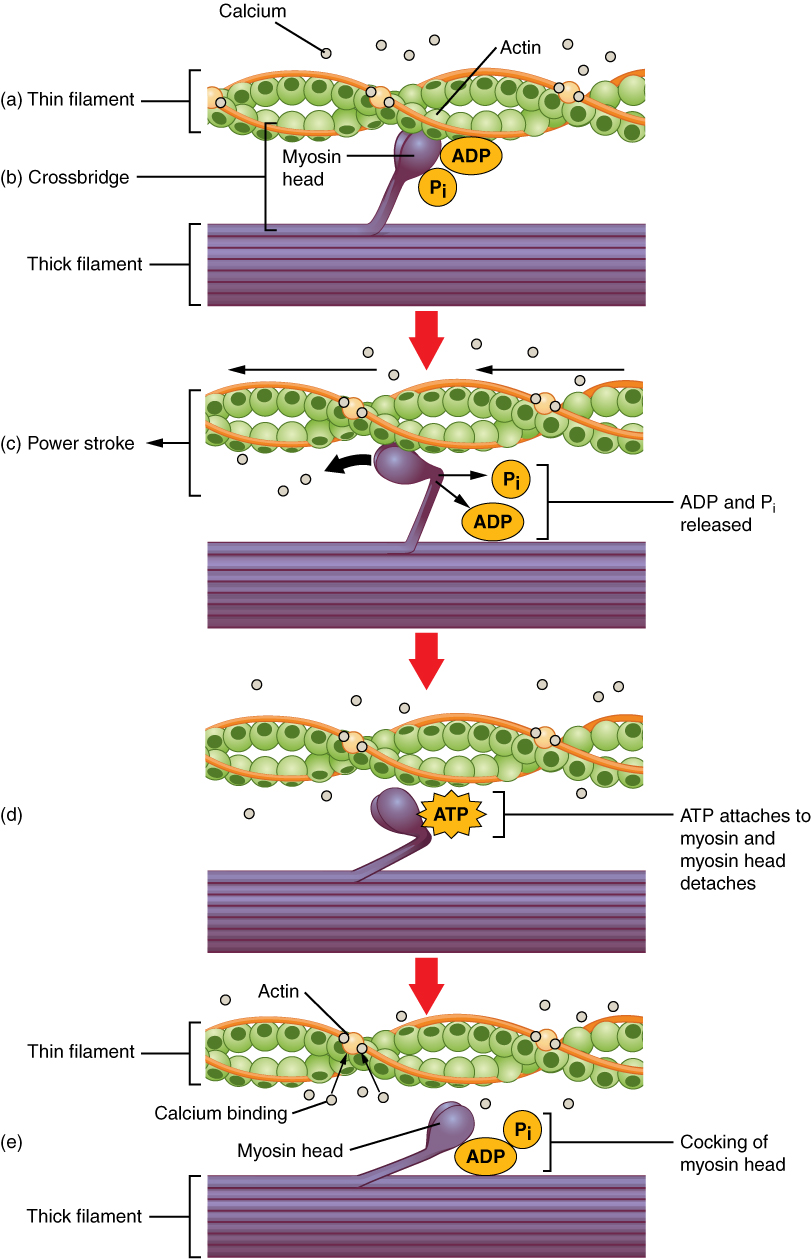
\includegraphics[width=0.7\linewidth]{./figures/locomotion/1008_Skeletal_Muscle_Contraction} 

}

\caption{\href{https://upload.wikimedia.org/wikipedia/commons/2/24/1008_Skeletal_Muscle_Contraction.jpg}{Crossbridge cycling.}}\label{fig:crossbridge}
\end{figure}

Crossbridge cycling is able to continue as long as there are sufficient amounts of ATP and Ca\textsuperscript{2+} in the cytoplasm. Termination of crossbridge cycling can occur when Ca\textsuperscript{2+} is actively pumped back into the sarcoplasmic reticulum. When Ca\textsuperscript{2+} is no longer present on the thin filament, the tropomyosin changes conformation back to its previous state so as to block the binding sites again. The myosin ceases binding to the thin filament, and the muscle relaxes. The Ca\textsuperscript{2+} ions leave the troponin molecule in order to maintain the Ca\textsuperscript{2+} ion concentration in the sarcoplasm. The active pumping of Ca\textsuperscript{2+} ions into the sarcoplasmic reticulum creates a deficiency in the fluid around the myofibrils. This causes the removal of Ca\textsuperscript{2+} ions from the troponin. Thus, the tropomyosin-troponin complex again covers the binding sites on the actin filaments and contraction ceases.

The strength of skeletal muscle contractions can be broadly separated into twitch, summation, and tetanus. A twitch is a single contraction and relaxation cycle produced by an action potential within the muscle fiber itself. The time between a stimulus to the motor nerve and the subsequent contraction of the innervated muscle is called the latent period, which usually takes about 10 ms and is caused by the time taken for nerve action potential to propagate, the time for chemical transmission at the neuromuscular junction, then the subsequent steps in excitation-contraction coupling.

If another muscle action potential were to be produced before the complete relaxation of a muscle twitch, then the next twitch will simply sum onto the previous twitch, thereby producing a summation. Summation can be achieved in two ways: frequency summation and multiple fiber summation. In frequency summation, the force exerted by the skeletal muscle is controlled by varying the frequency at which action potentials are sent to muscle fibers. Action potentials do not arrive at muscles synchronously, and, during a contraction, some fraction of the fibers in the muscle will be firing at any given time. In a typical circumstance, when humans are exerting their muscles as hard as they are consciously able, roughly one-third of the fibers in each of those muscles will fire at once, though this ratio can be affected by various physiological and psychological factors (including Golgi tendon organs and Renshaw cells). This `low' level of contraction is a protective mechanism to prevent avulsion of the tendon---the force generated by a 95\% contraction of all fibers is sufficient to damage the body. In multiple fiber summation, if the central nervous system sends a weak signal to contract a muscle, the smaller motor units, being more excitable than the larger ones, are stimulated first. As the strength of the signal increases, more motor units are excited in addition to larger ones, with the largest motor units having as much as 50 times the contractile strength as the smaller ones. As more and larger motor units are activated, the force of muscle contraction becomes progressively stronger. A concept known as the size principle, allows for a gradation of muscle force during weak contraction to occur in small steps, which then become progressively larger when greater amounts of force are required.

Finally, if the frequency of muscle action potentials increases such that the muscle contraction reaches its peak force and plateaus at this level, then the contraction is a tetanus.

Length-tension relationship relates the strength of an isometric contraction to the length of the muscle at which the contraction occurs. Muscles operate with greatest active tension when close to an ideal length (often their resting length). When stretched or shortened beyond this (whether due to the action of the muscle itself or by an outside force), the maximum active tension generated decreases. This decrease is minimal for small deviations, but the tension drops off rapidly as the length deviates further from the ideal. Due to the presence of elastic proteins within a muscle cell (such as titin) and extracellular matrix, as the muscle is stretched beyond a given length, there is an entirely passive tension, which opposes lengthening. Combined together, there is a strong resistance to lengthening an active muscle far beyond the peak of active tension.

Force--velocity relationship relates the speed at which a muscle changes its length (usually regulated by external forces, such as load or other muscles) to the amount of force that it generates. Force declines in a hyperbolic fashion relative to the isometric force as the shortening velocity increases, eventually reaching zero at some maximum velocity. The reverse holds true for when the muscle is stretched -- force increases above isometric maximum, until finally reaching an absolute maximum. This intrinsic property of active muscle tissue plays a role in the active damping of joints that are actuated by simultaneously-active opposing muscles. In such cases, the force-velocity profile enhances the force produced by the lengthening muscle at the expense of the shortening muscle. This favoring of whichever muscle returns the joint to equilibrium effectively increases the damping of the joint. Moreover, the strength of the damping increases with muscle force. The motor system can thus actively control joint damping via the simultaneous contraction (co-contraction) of opposing muscle groups.

\hypertarget{smooth-muscle}{%
\subsection{Smooth Muscle}\label{smooth-muscle}}

Smooth muscles can be divided into two subgroups: single-unit (unitary) and multi-unit. Single-unit smooth muscle cells can be found in the gut and blood vessels. Because these cells are linked together by gap junctions, they are able to contract as a syncytium. Single-unit smooth muscle cells contract myogenically, which can be modulated by the autonomic nervous system.

Unlike single-unit smooth muscle cells, multi-unit smooth muscle cells are found in the muscle of the eye and in the base of hair follicles. Multi-unit smooth muscle cells contract by being separately stimulated by nerves of the autonomic nervous system. As such, they allow for fine control and gradual responses, much like motor unit recruitment in skeletal muscle.

The contractile activity of smooth muscle cells is influenced by multiple inputs such as spontaneous electrical activity, neural and hormonal inputs, local changes in chemical composition, and stretch. This is in contrast to the contractile activity of skeletal muscle cells, which relies on a single neural input. Some types of smooth muscle cells are able to generate their own action potentials spontaneously, which usually occur following a pacemaker potential or a slow wave potential. These action potentials are generated by the influx of extracellular Ca\textsuperscript{2+} , and not Na\textsuperscript{+}. Like skeletal muscles, cytosolic Ca\textsuperscript{2+} ions are also required for crossbridge cycling in smooth muscle cells.

The two sources for cytosolic Ca\textsuperscript{2+} in smooth muscle cells are the extracellular Ca\textsuperscript{2+} entering through calcium channels and the Ca\textsuperscript{2+} ions that are released from the sarcoplasmic reticulum. The elevation of cytosolic Ca\textsuperscript{2+} results in more Ca\textsuperscript{2+} binding to calmodulin, which then binds and activates myosin light-chain kinase. The calcium-calmodulin-myosin light-chain kinase complex phosphorylates myosin on the 20 kilodalton (kDa) myosin light chains on amino acid residue-serine 19, initiating contraction and activating the myosin ATPase. Unlike skeletal muscle cells, smooth muscle cells lack troponin, even though they contain the thin filament protein tropomyosin and other notable proteins -- caldesmon and calponin. Thus, smooth muscle contractions are initiated by the Ca\textsuperscript{2+} -activated phosphorylation of myosin rather than Ca\textsuperscript{2+} binding to the troponin complex that regulates myosin binding sites on actin like in skeletal and cardiac muscles.

Termination of crossbridge cycling (and leaving the muscle in latch-state) occurs when myosin light chain phosphatase removes the phosphate groups from the myosin heads. Phosphorylation of the 20 kDa myosin light chains correlates well with the shortening velocity of smooth muscle. During this period, there is a rapid burst of energy utilization as measured by oxygen consumption. Within a few minutes of initiation, the calcium level markedly decreases, the 20 kDa myosin light chains' phosphorylation decreases, and energy utilization decreases; however, force in tonic smooth muscle is maintained. During contraction of muscle, rapidly cycling crossbridges form between activated actin and phosphorylated myosin, generating force. It is hypothesized that the maintenance of force results from dephosphorylated ``latch-bridges'' that slowly cycle and maintain force. A number of kinases such as rho kinase, ZIP kinase, and protein kinase C are believed to participate in the sustained phase of contraction, and Ca\textsuperscript{2+} flux may be significant.

Although smooth muscle contractions are myogenic, the rate and strength of their contractions can be modulated by the autonomic nervous system. Postganglionic nerve fibers of parasympathetic nervous system release the neurotransmitter acetylcholine, which binds to muscarinic acetylcholine receptors (mAChRs) on smooth muscle cells. These receptors are metabotropic, or G-protein coupled receptors that initiate a second messenger cascade. Conversely, postganglionic nerve fibers of the sympathetic nervous system release the neurotransmitters epinephrine and norepinephrine, which bind to adrenergic receptors that are also metabotropic. The exact effects on the smooth muscle depend on the specific characteristics of the receptor activated---both parasympathetic input and sympathetic input can be either excitatory (contractile) or inhibitory (relaxing).

\hypertarget{cardiac-muscle}{%
\subsection{Cardiac Muscle}\label{cardiac-muscle}}

There are two types of cardiac muscle cells: autorhythmic and contractile. Autorhythmic cells do not contract, but instead set the pace of contraction for other cardiac muscle cells, which can be modulated by the autonomic nervous system. In contrast, contractile muscle cells (cardiomyocytes) constitute the majority of the heart muscle and are able to contract.

Unlike skeletal muscle, excitation--contraction coupling in cardiac muscle is thought to depend primarily on a mechanism called calcium-induced calcium release. Though the proteins involved are similar, the L-type calcium channels and ryanodine receptors (RyRs) are not physically coupled. Instead, RyRs are activated by a calcium trigger, which is brought about by the flow of Ca\textsuperscript{2+} through the L-type calcium channels. Furthermore, cardiac muscle tend to exhibit diad (or dyad) structures, rather than triads.

Excitation-contraction coupling in cardiac muscle cells occurs when an action potential is initiated by pacemaker cells in the sinoatrial node or Atrioventricular node and conducted to all cells in the heart via gap junctions. The action potential travels along the surface membrane into T-tubules (the latter are not seen in all cardiac cell types) and the depolarisation causes extracellular Ca\textsuperscript{2+} to enter the cell via L-type calcium channels and possibly sodium-calcium exchanger (NCX) during the early part of the plateau phase. This Ca\textsuperscript{2+} influx causes a small local increase in intracellular Ca\textsuperscript{2+} . The increase in Ca\textsuperscript{2+} is detected by ryanodine receptors in the membrane of the sarcoplasmic reticulum, which releases Ca\textsuperscript{2+} in a positive feedback physiological response. This positive feedback is known as calcium-induced calcium release and gives rise to calcium sparks (Ca\textsuperscript{2+} sparks). The spatial and temporal summation of \textasciitilde30,000 Ca\textsuperscript{2+} sparks gives a cell-wide increase in cytoplasmic calcium concentration. The increase in cytosolic calcium following the flow of calcium through the cell membrane and sarcoplasmic reticulum is moderated by calcium buffers, which bind a large proportion of intracellular calcium. As a result, a large increase in total calcium leads to a relatively small rise in free Ca\textsuperscript{2+} .

Following systole, intracellular calcium is taken up by the sarco/endoplasmic reticulum ATPase (SERCA) pump back into the sarcoplasmic reticulum ready for the next cycle to begin. Calcium is also ejected from the cell mainly by the sodium-calcium exchanger (NCX) and, to a lesser extent, a plasma membrane calcium ATPase. Some calcium is also taken up by the mitochondria. An enzyme, phospholamban, serves as a brake for SERCA. At low heart rates, phospholamban is active and slows down the activity of the ATPase so that Ca\textsuperscript{2+} does not have to leave the cell entirely. At high heart rates, phospholamban is phosphorylated and deactivated thus taking most Ca\textsuperscript{2+}from the cytoplasm back into the sarcoplasmic reticulum. Once again, calcium buffers moderate this fall in Ca\textsuperscript{2+} concentration, permitting a relatively small decrease in free Ca\textsuperscript{2+} concentration in response to a large change in total calcium. The falling Ca\textsuperscript{2+} concentration allows the troponin complex to dissociate from the actin filament thereby ending contraction. The heart relaxes, allowing the ventricles to fill with blood and begin the cardiac cycle again.

\hypertarget{the-muscular-systems-of-invertebrates}{%
\subsection{The Muscular Systems of Invertebrates}\label{the-muscular-systems-of-invertebrates}}

In annelids such as earthworms and leeches, circular and longitudinal muscles cells form the body wall of these animals and are responsible for their movement. In an earthworm that is moving through a soil, for example, contractions of circular and longitudinal muscles occur reciprocally while the coelomic fluid serves as a hydroskeleton by maintaining turgidity of the earthworm. When the circular muscles in the anterior segments contract, the anterior portion of animal's body begins to constrict radially, which pushes the incompressible coelomic fluid forward and increasing the length of the animal. As a result, the front end of the animal moves forward. As the front end of the earthworm becomes anchored and the circular muscles in the anterior segments become relaxed, a wave of longitudinal muscle contractions passes backwards, which pulls the rest of animal's trailing body forward. These alternating waves of circular and longitudinal contractions is called peristalsis, which underlies the creeping movement of earthworms.

Invertebrates such as annelids, mollusks, and nematodes, possess obliquely striated muscles, which contain bands of thick and thin filaments that are arranged helically rather than transversely, like in vertebrate skeletal or cardiac muscles. In bivalves, the obliquely striated muscles can maintain tension over long periods without using too much energy. Bivalves use these muscles to keep their shells closed.

Advanced insects such as wasps, flies, bees, and beetles possess asynchronous muscles that constitute the flight muscles in these animals. These flight muscles are often called fibrillar muscles because they contain myofibrils that are thick and conspicuous. A remarkable feature of these muscles is that they do not require stimulation for each muscle contraction. Hence, they are called asynchronous muscles because the number of contractions in these muscles do not correspond (or synchronize) with the number of action potentials. For example, a wing muscle of a tethered fly may receive action potentials at a frequency of 3 Hz but it is able to beat at a frequency of 120 Hz. The high frequency beating is made possible because the muscles are connected to a resonant system, which is driven to a natural frequency of vibration.


